\section{Issues when compiling from sources}

\begin{frame}
    \frametitle{Compile from source process}

    After the distribution source is found, follows the following steps to compile.

    \begin{enumerate}
        \item Find installing steps in \alert{\texttt{readme.md}}, \alert{\texttt{README}}, or \alert{\texttt{INSTALL}}.
        \item If not, find \texttt{configure} to execute.
        \item If not, find custom installing scripts like \alert{\texttt{bootstrap}}, \alert{\texttt{autogen}} often in \textit{Bash} or \textit{Shell} syntax.
        \item If not, find corresponding configuration files of each build systems. If identified, use the convension compiling commands.
        \item In the build process, the build system might inform about missing dependency. Find the distribution source and repeat the process.
    \end{enumerate}
\end{frame}

\subsection{Distinguish build systems}

\begin{frame}
    \frametitle{Example: \texttt{pcre2}}

    \begin{center}
        \begin{tikzpicture}
            \node[anchor=south west,inner sep=0] at (0,0) {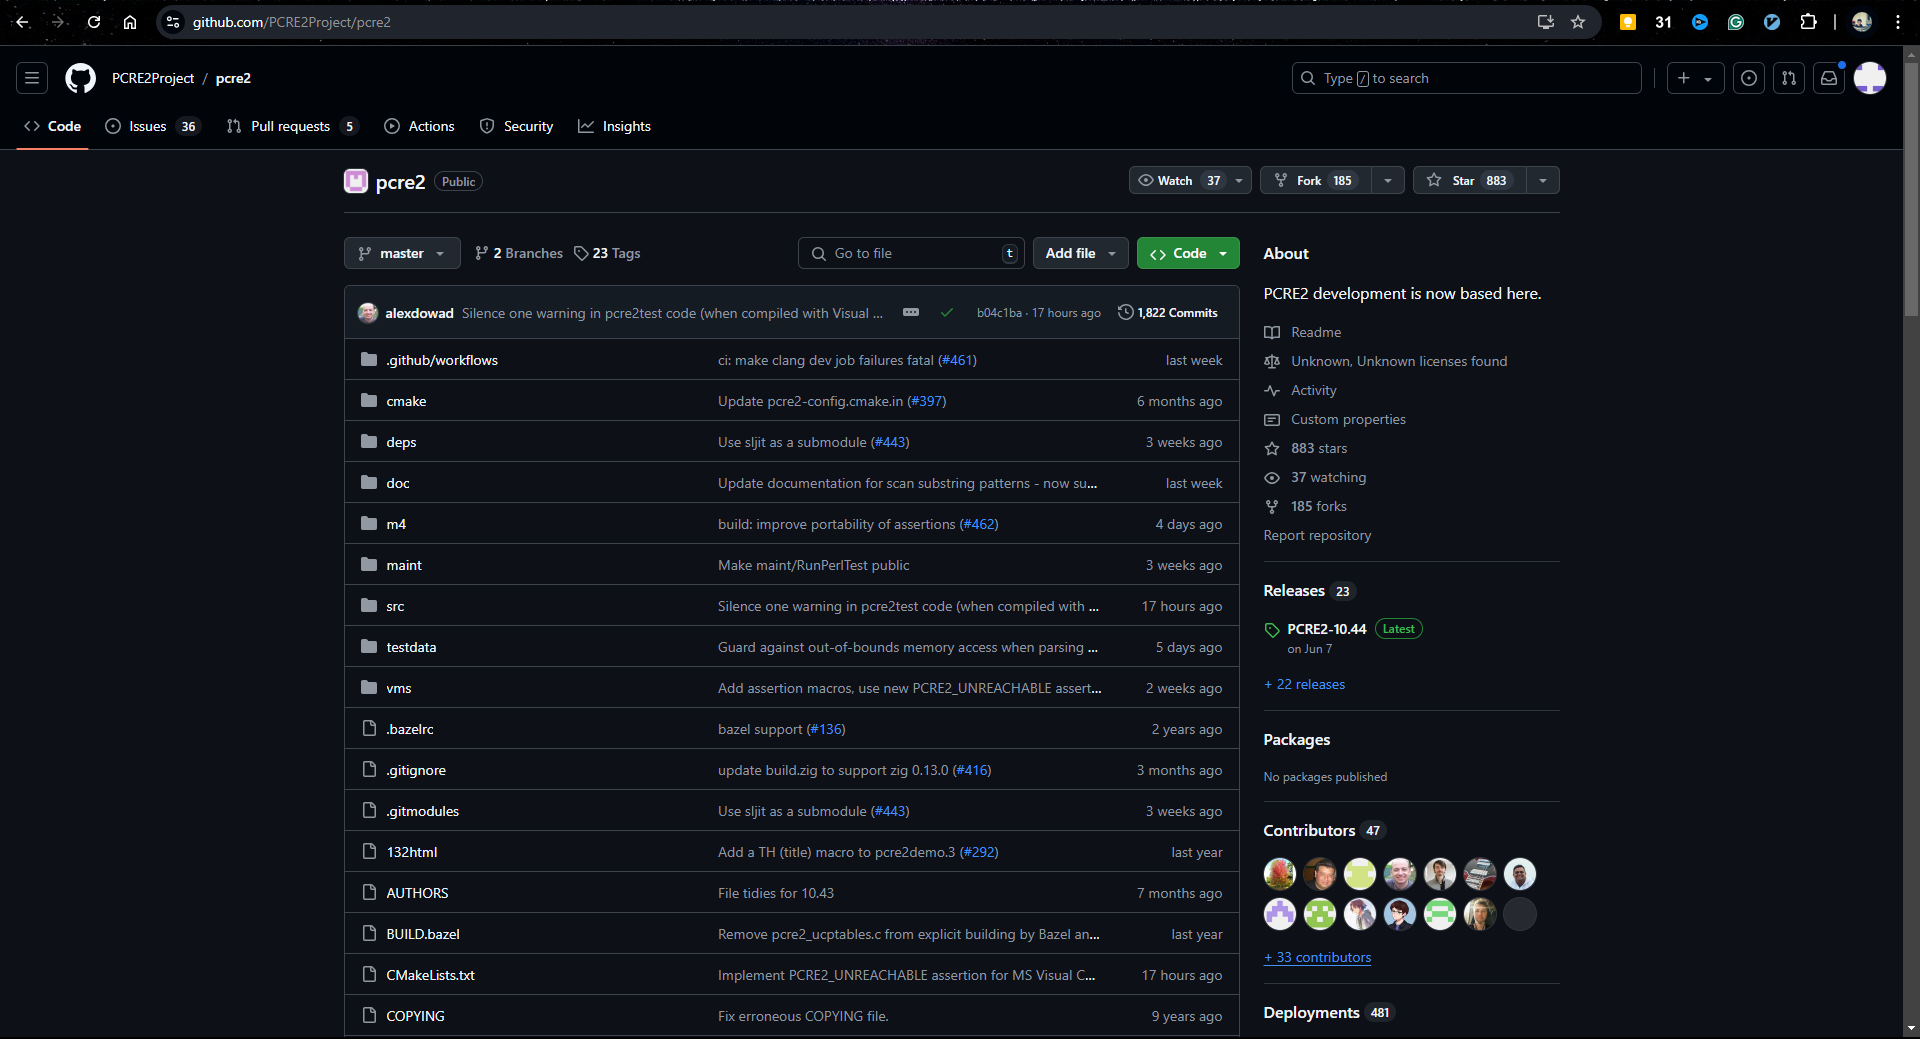
\includegraphics[width=\textwidth=0.8]{../figure/pcre2_1.png}};
            \draw[red,line width=0.1mm] (2.1,0.51) rectangle (7.9,0.3);
        \end{tikzpicture}
    \end{center}
\end{frame}

\begin{frame}
    \frametitle{Example: \texttt{pcre2}}

    \begin{center}
        \begin{tikzpicture}
            \node[anchor=south west,inner sep=0] at (0,0) {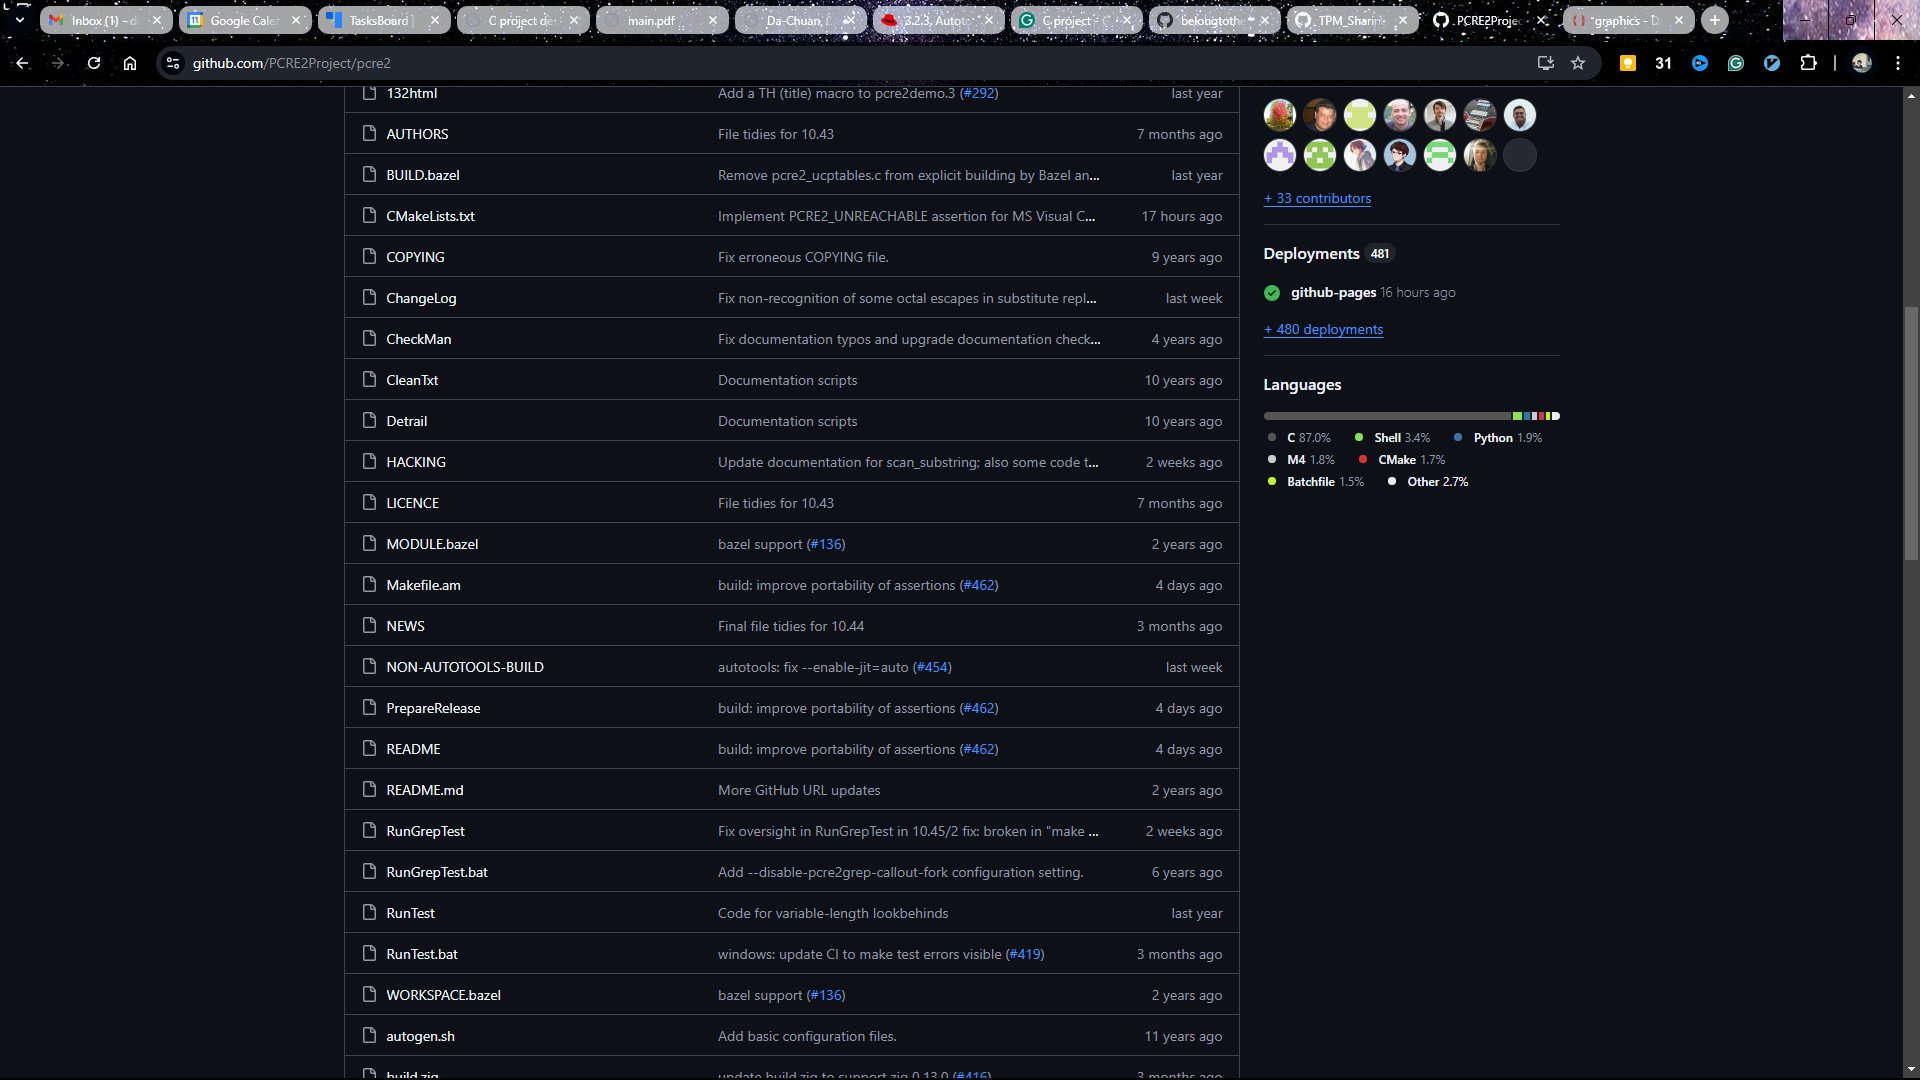
\includegraphics[width=\textwidth=0.8]{../figure/pcre2_2.png}};
            \draw[red,line width=0.1mm] (2.1,5.51) rectangle (7.9,5.3);
            \draw[red,line width=0.1mm] (2.1,3.21) rectangle (7.9,3.0);
            \draw[red,line width=0.1mm] (2.1,2.21) rectangle (7.9,2.0);
            \draw[red,line width=0.1mm] (2.1,1.93) rectangle (7.9,1.73);
            \draw[red,line width=0.1mm] (2.1,0.40) rectangle (7.9,0.20);
        \end{tikzpicture}
    \end{center}
\end{frame}

\begin{frame}
    \frametitle{Example: \texttt{pcre2}}

    \begin{center}
        \begin{tikzpicture}
            \node[anchor=south west,inner sep=0] at (0,0) {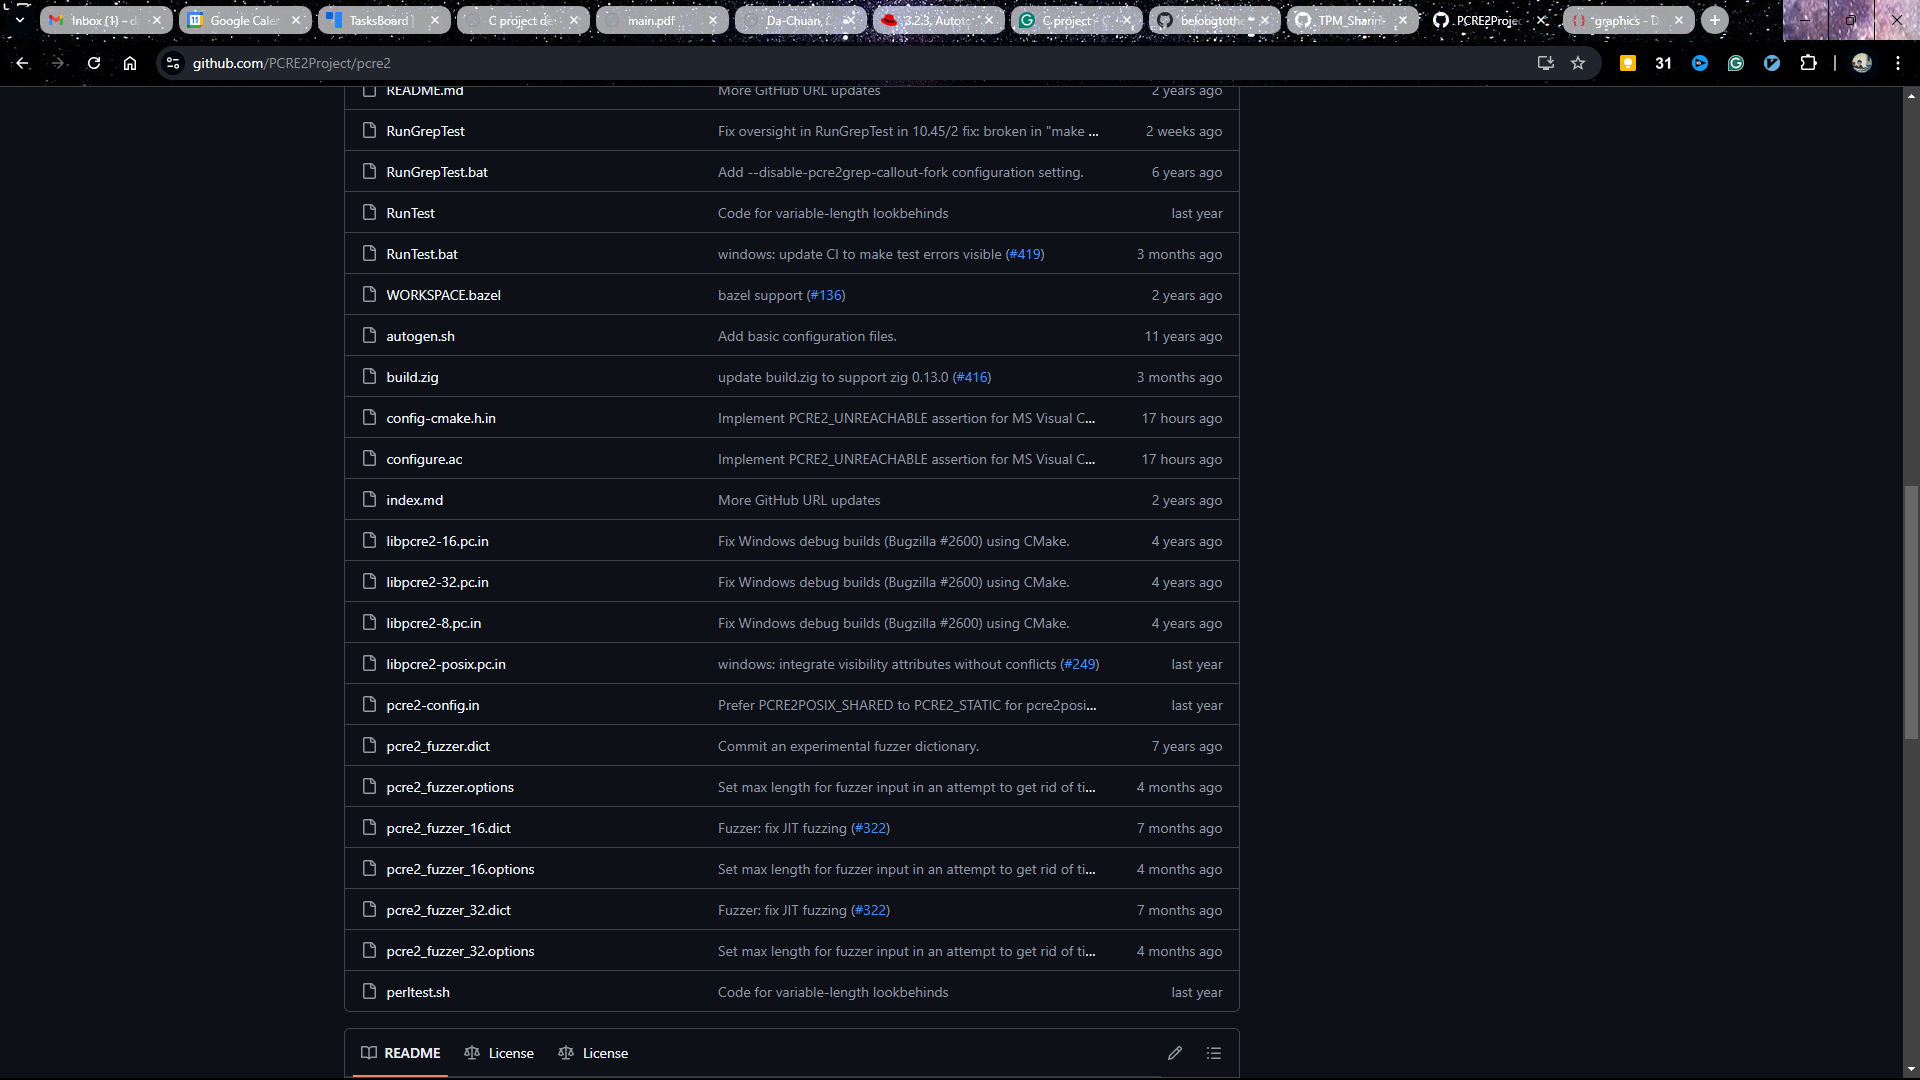
\includegraphics[width=\textwidth=0.8]{../figure/pcre2_3.png}};
            \draw[red,line width=0.1mm] (2.1,4.80) rectangle (7.9,4.60);
            \draw[red,line width=0.1mm] (2.1,4.00) rectangle (7.9,3.80);
        \end{tikzpicture}
    \end{center}
\end{frame}

\begin{frame}
    \frametitle{Example: \texttt{pcre2}}

    The above project structure is an example of source code distribution for development. Boxed files might not exist in the release version, and some new files might appear. Therefore, the same analysis on how to build the project should be done in the same way but after uncompressing the distributed software.

    The \texttt{pcre2} example should actually be compiled with the following commands:

    \begin{figure}[H]
        \centering
        \hfill
        \begin{minipage}{.8\textwidth}
            \inputminted[
                mathescape,
                linenos,
                autogobble,
                fontsize=\scriptsize,
            ]{bash}{E:\\GitHub\\presentation_in_LaTeX\\c_project_development\\script\\build_pcre2.sh}
        \end{minipage}
        \hfill
        \caption*{Code to compile lib \texttt{pcre2} with custom flags.}
    \end{figure}
\end{frame}

\begin{frame}
    \frametitle{Exercise: Build \texttt{pcre2}}

    Step 1: Find the distribution.

    \begin{figure}[H]
        \centering
        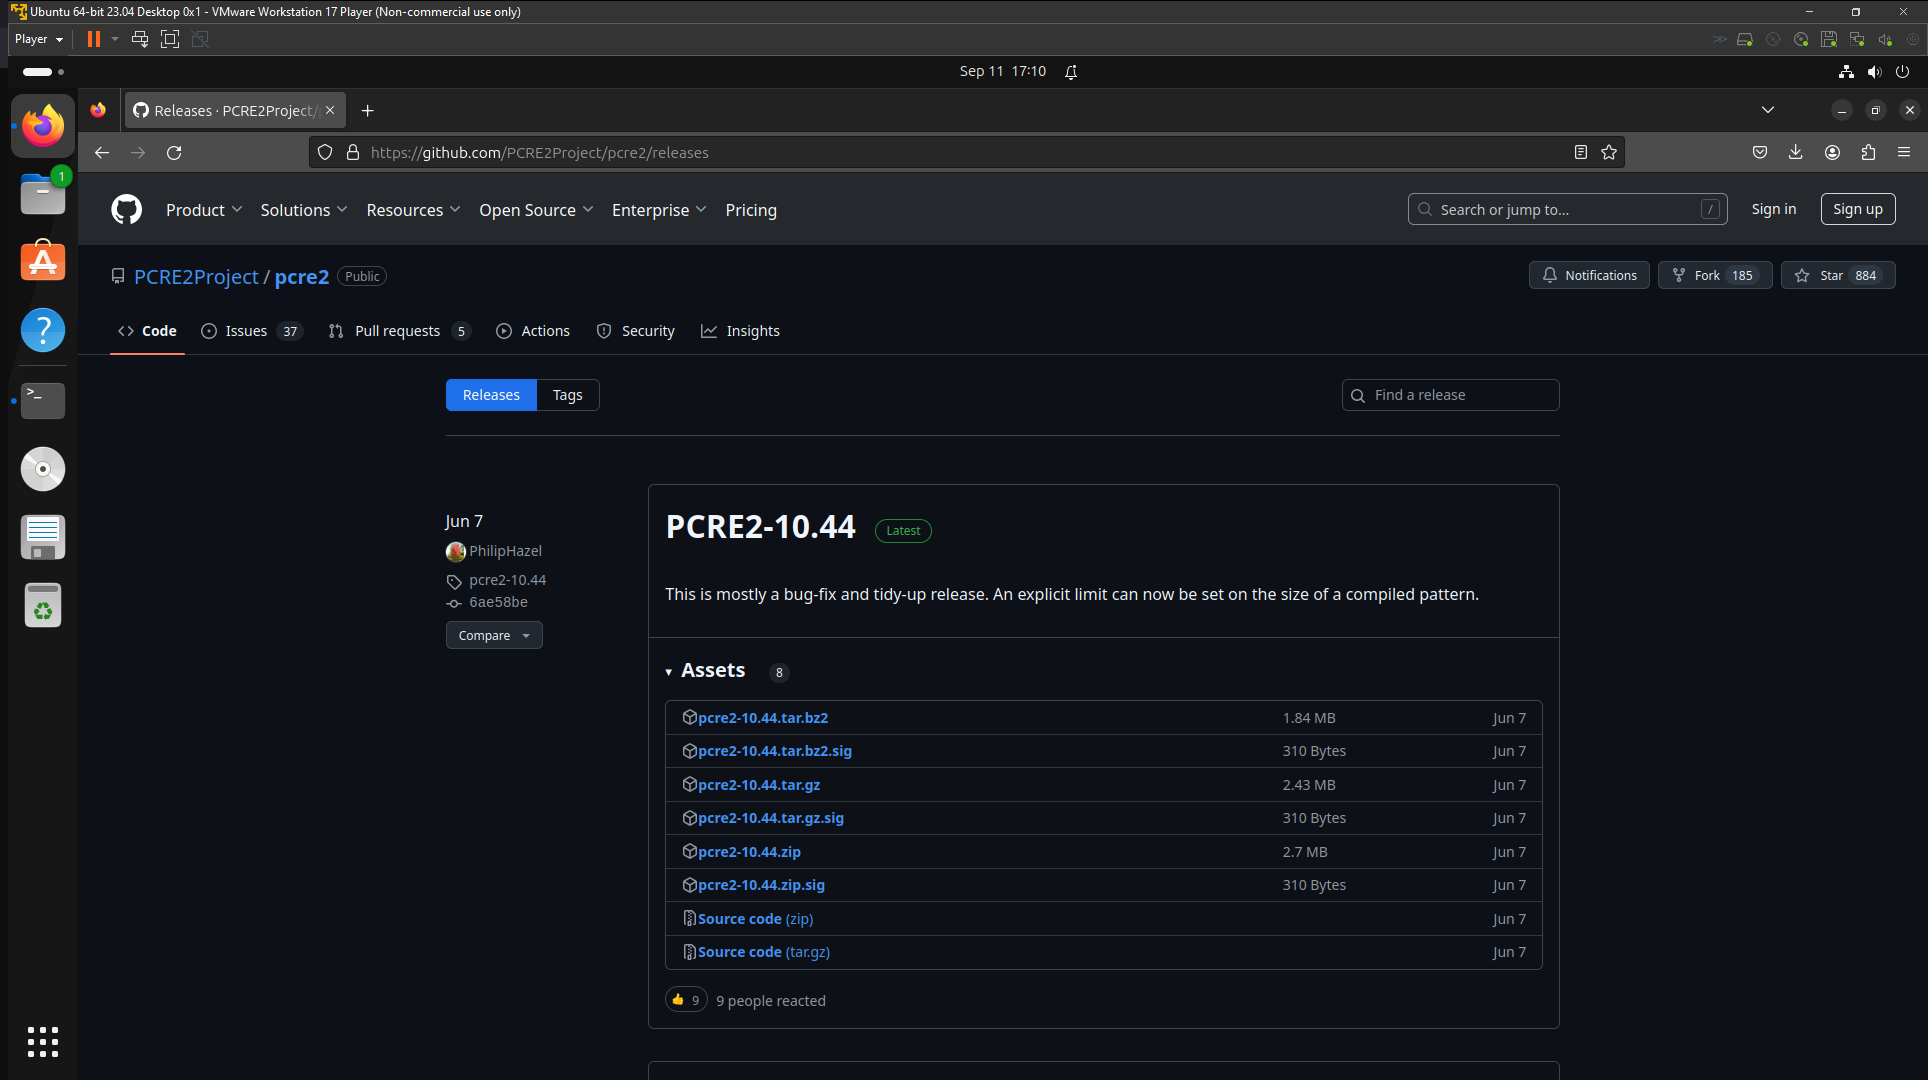
\includegraphics[width=0.9\textwidth]{../figure/pcre2_build_1.png}
    \end{figure}

\end{frame}

\begin{frame}
    \frametitle{Exercise: Build \texttt{pcre2}}

    Step 2: Copy the download link. (for downloading)

    \begin{figure}[H]
        \centering
        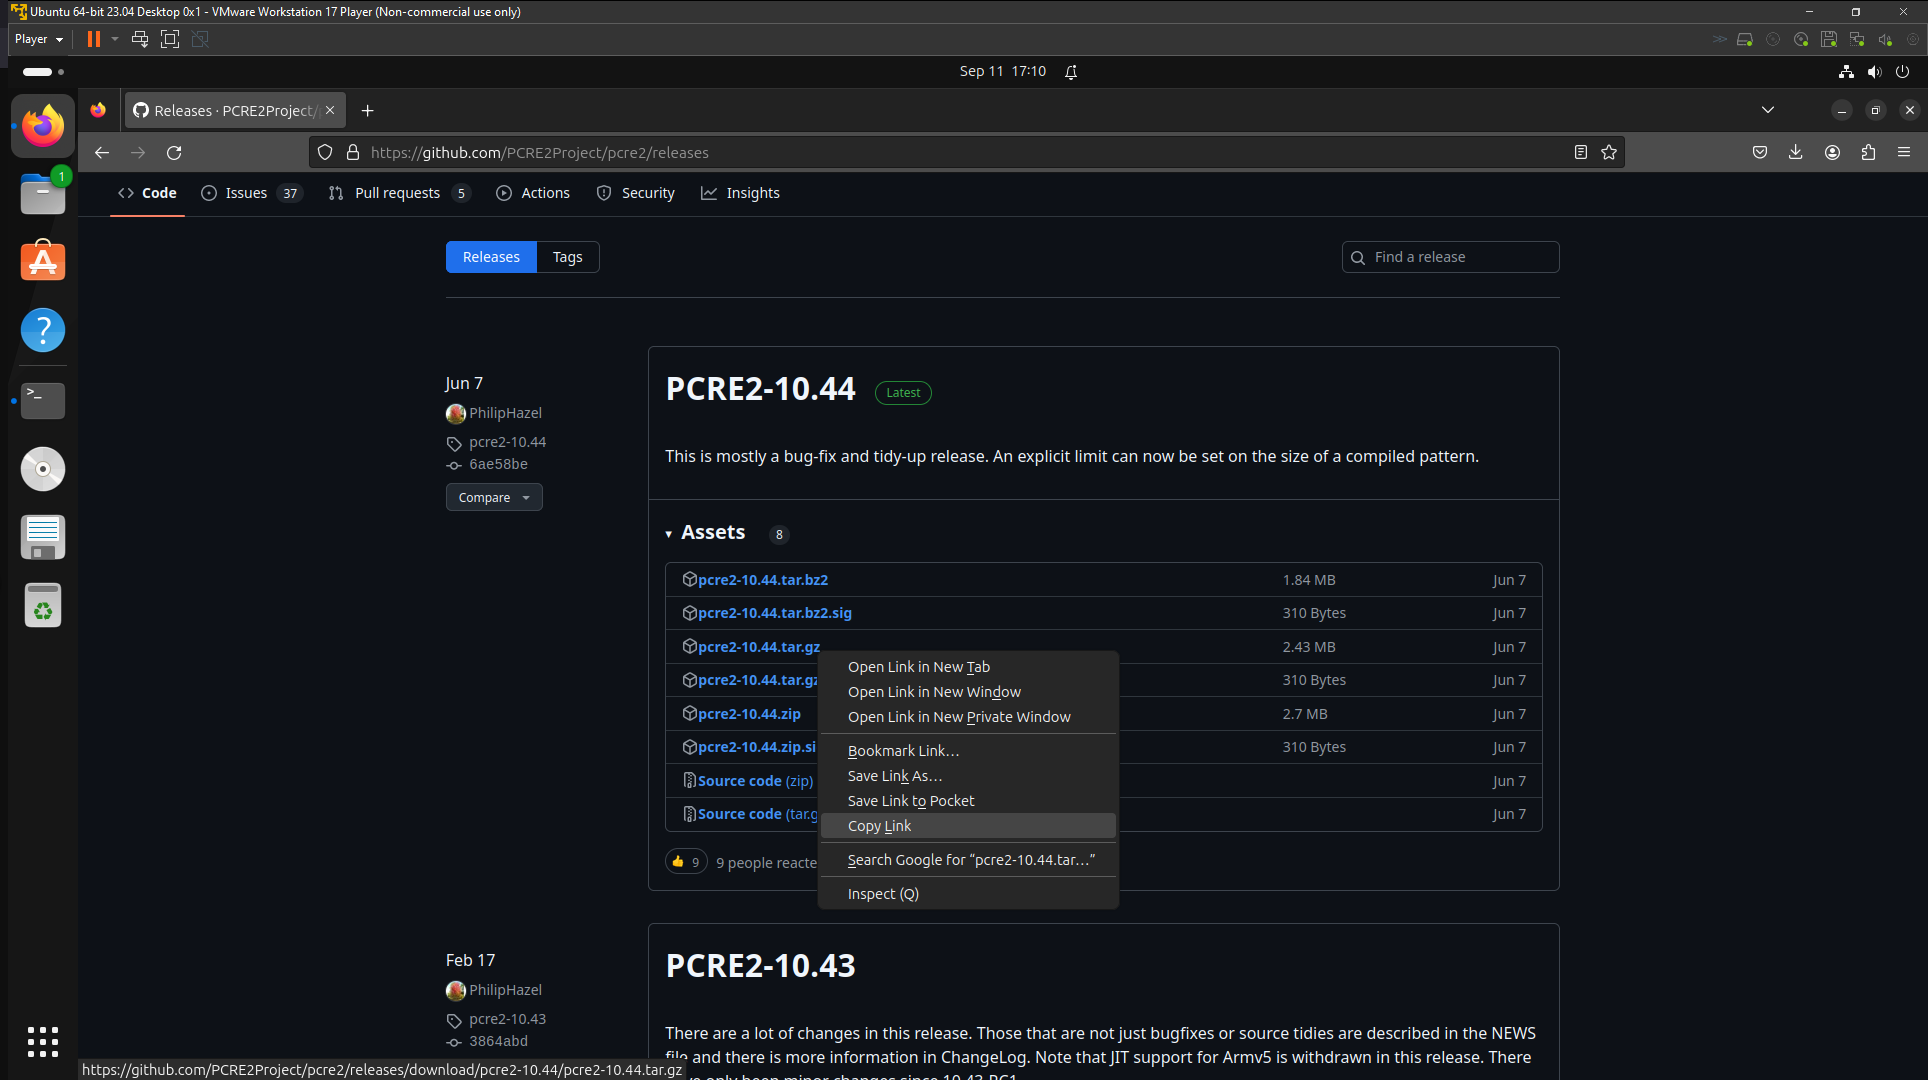
\includegraphics[width=0.9\textwidth]{../figure/pcre2_build_2.png}
    \end{figure}

\end{frame}

\begin{frame}
    \frametitle{Exercise: Build \texttt{pcre2}}

    Step 3: Download the compressed source code.

    \begin{figure}[H]
        \centering
        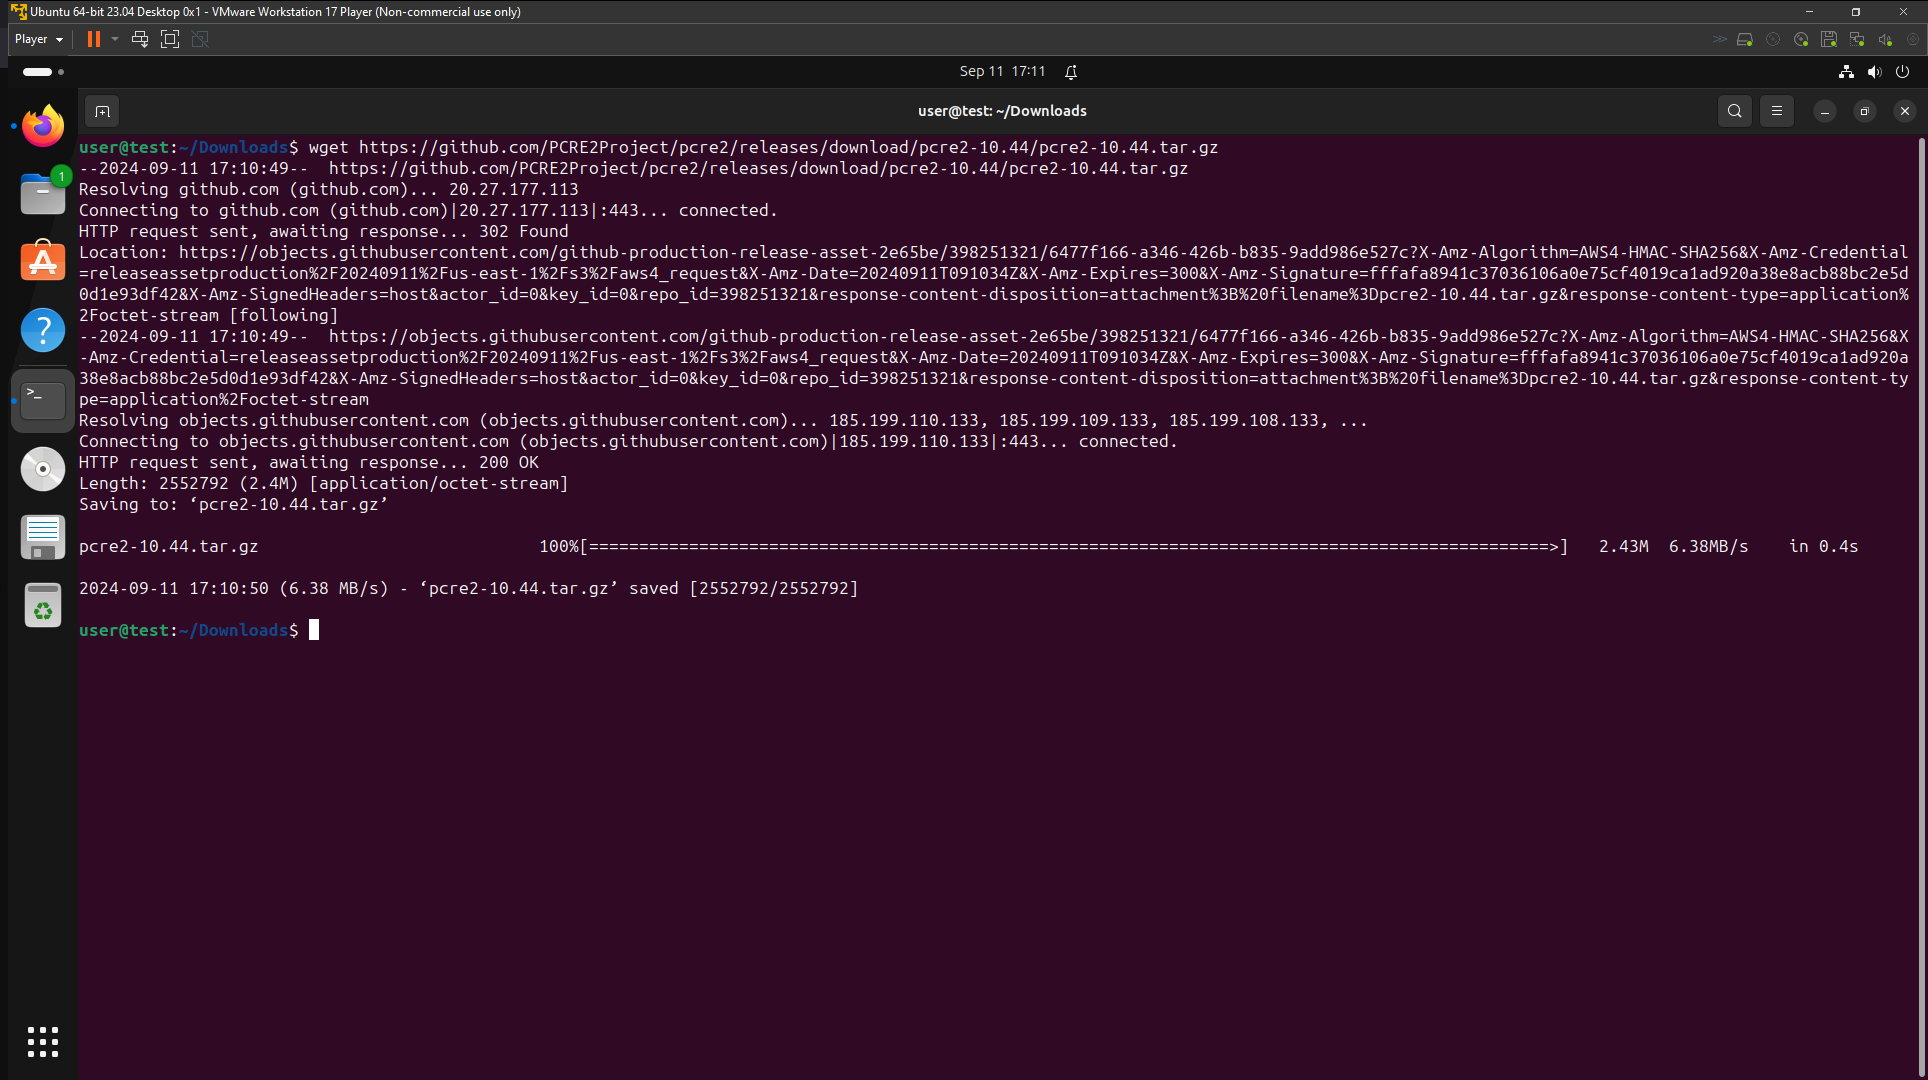
\includegraphics[width=0.9\textwidth]{../figure/pcre2_build_3.png}
    \end{figure}

\end{frame}

\begin{frame}
    \frametitle{Exercise: Build \texttt{pcre2}}

    Step 4: Create a directory with custom naming and uncompress the source code into it. Notice that there are binary \alert{\texttt{./configure}} existed, and can be used for building.

    \begin{figure}[H]
        \centering
        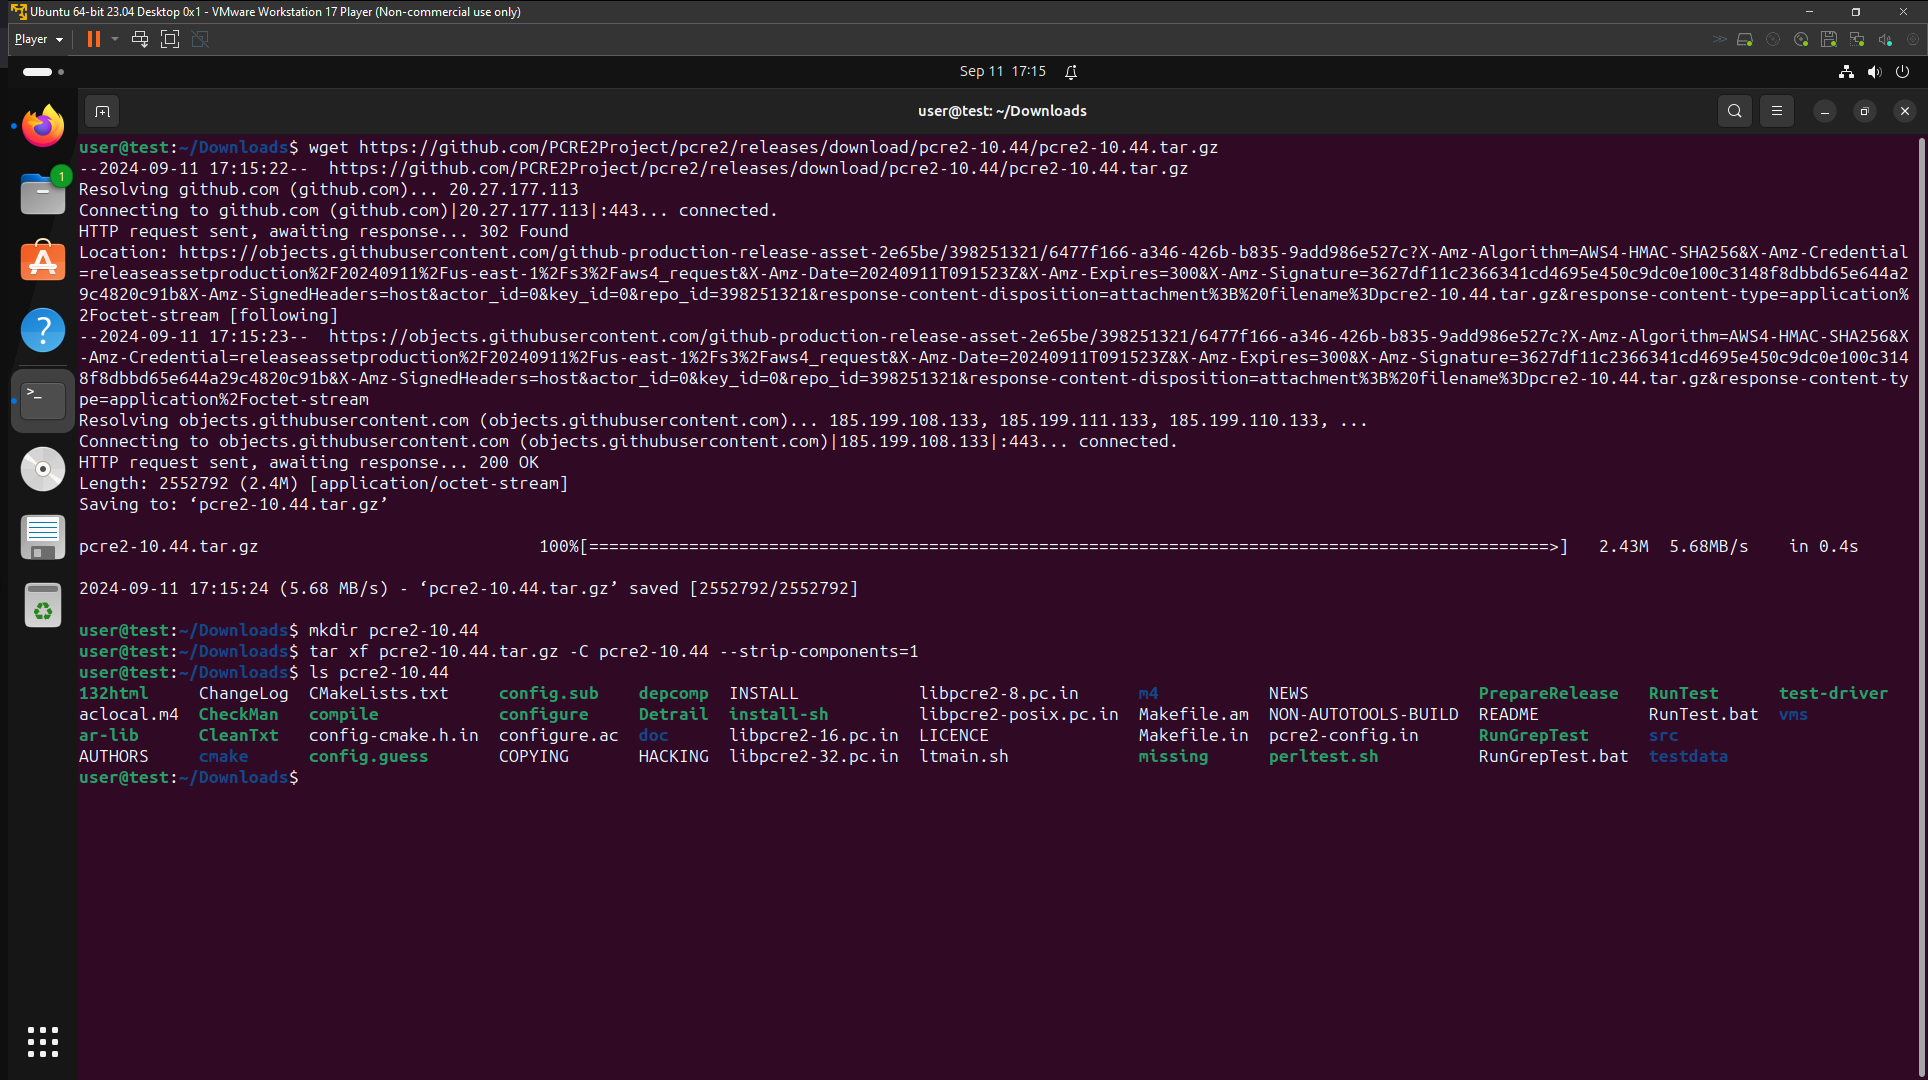
\includegraphics[width=0.9\textwidth]{../figure/pcre2_build_4.png}
    \end{figure}

\end{frame}

\begin{frame}
    \frametitle{Exercise: Build \texttt{pcre2}}

    Step 5: Execute \texttt{./configure} to configure files for building.

    \begin{figure}[H]
        \centering
        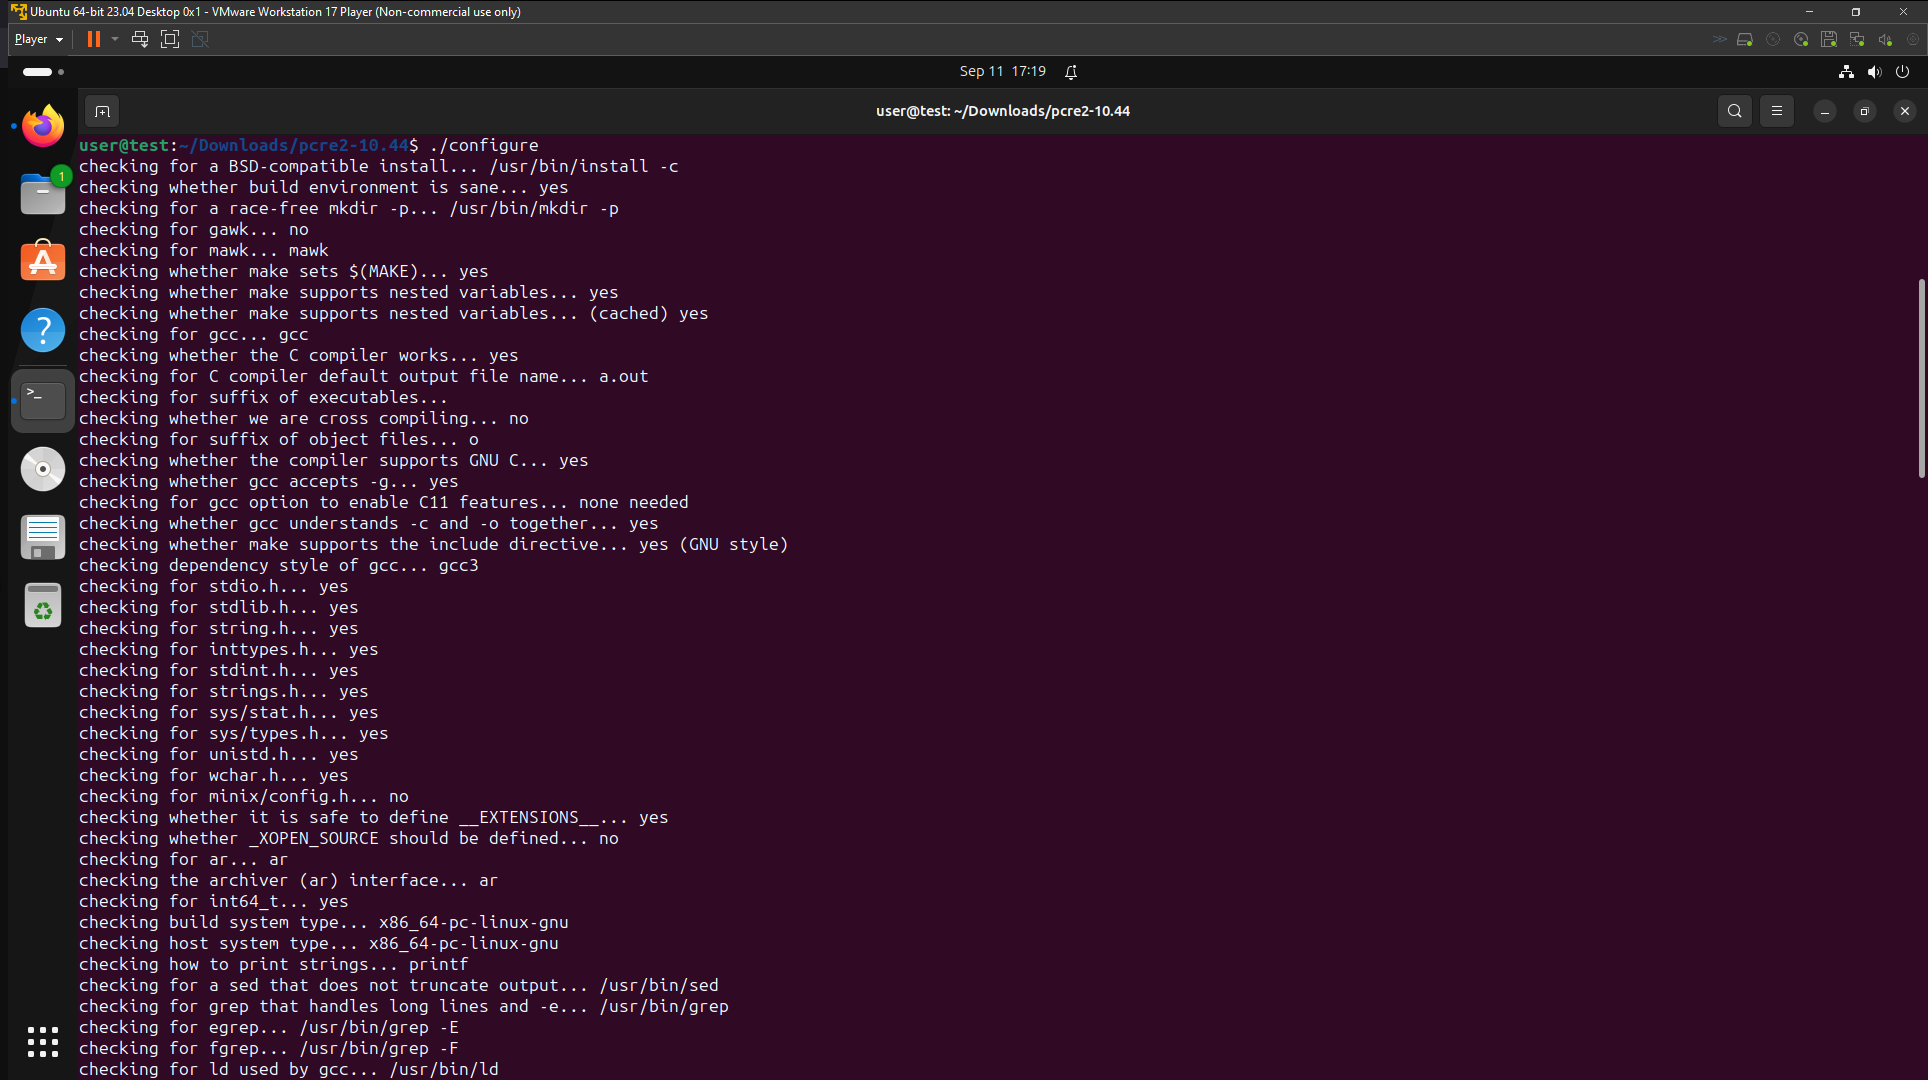
\includegraphics[width=0.9\textwidth]{../figure/pcre2_build_5.png}
    \end{figure}

\end{frame}

\begin{frame}
    \frametitle{Exercise: Build \texttt{pcre2}}

    Step 6: Make sure no error is shown in the output and execute \texttt{make} to build

    \begin{figure}[H]
        \centering
        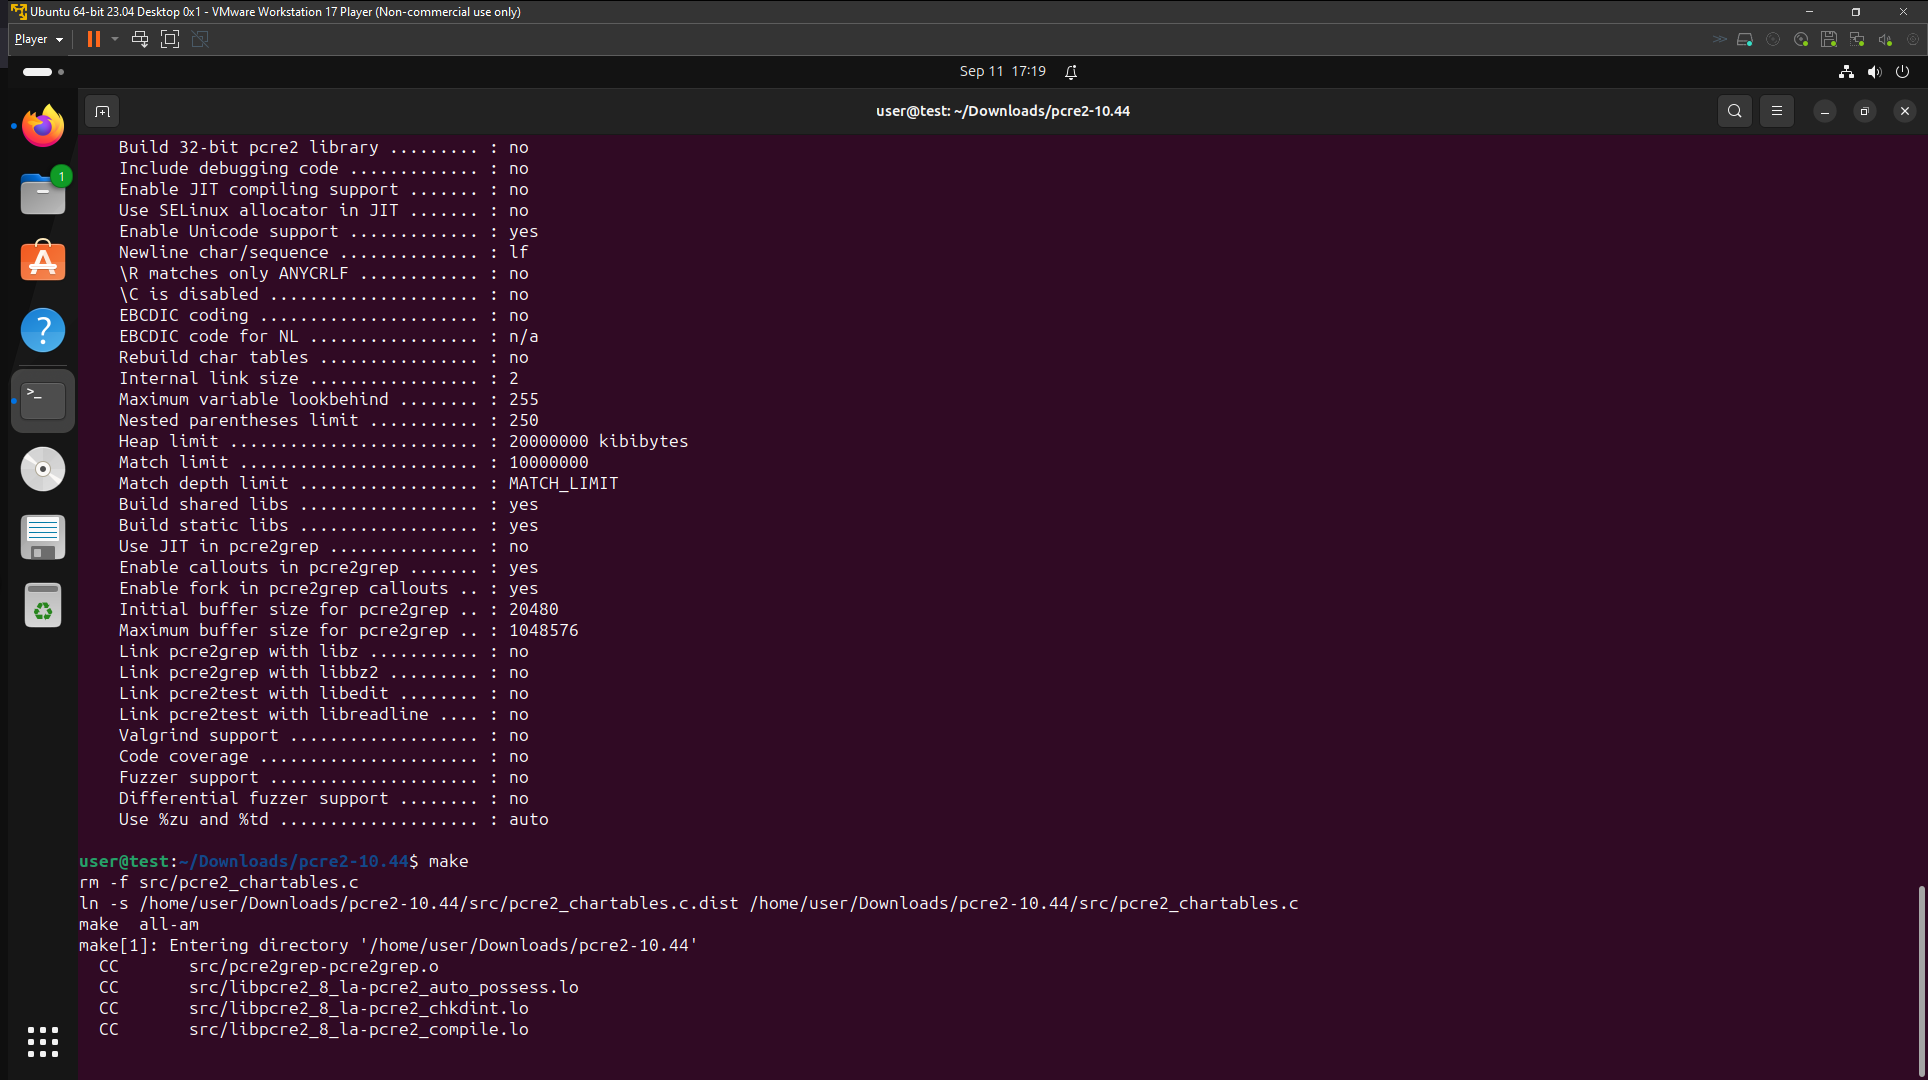
\includegraphics[width=0.9\textwidth]{../figure/pcre2_build_6.png}
    \end{figure}

\end{frame}

\begin{frame}
    \frametitle{Exercise: Build \texttt{pcre2}}

    \begin{figure}[H]
        \centering
        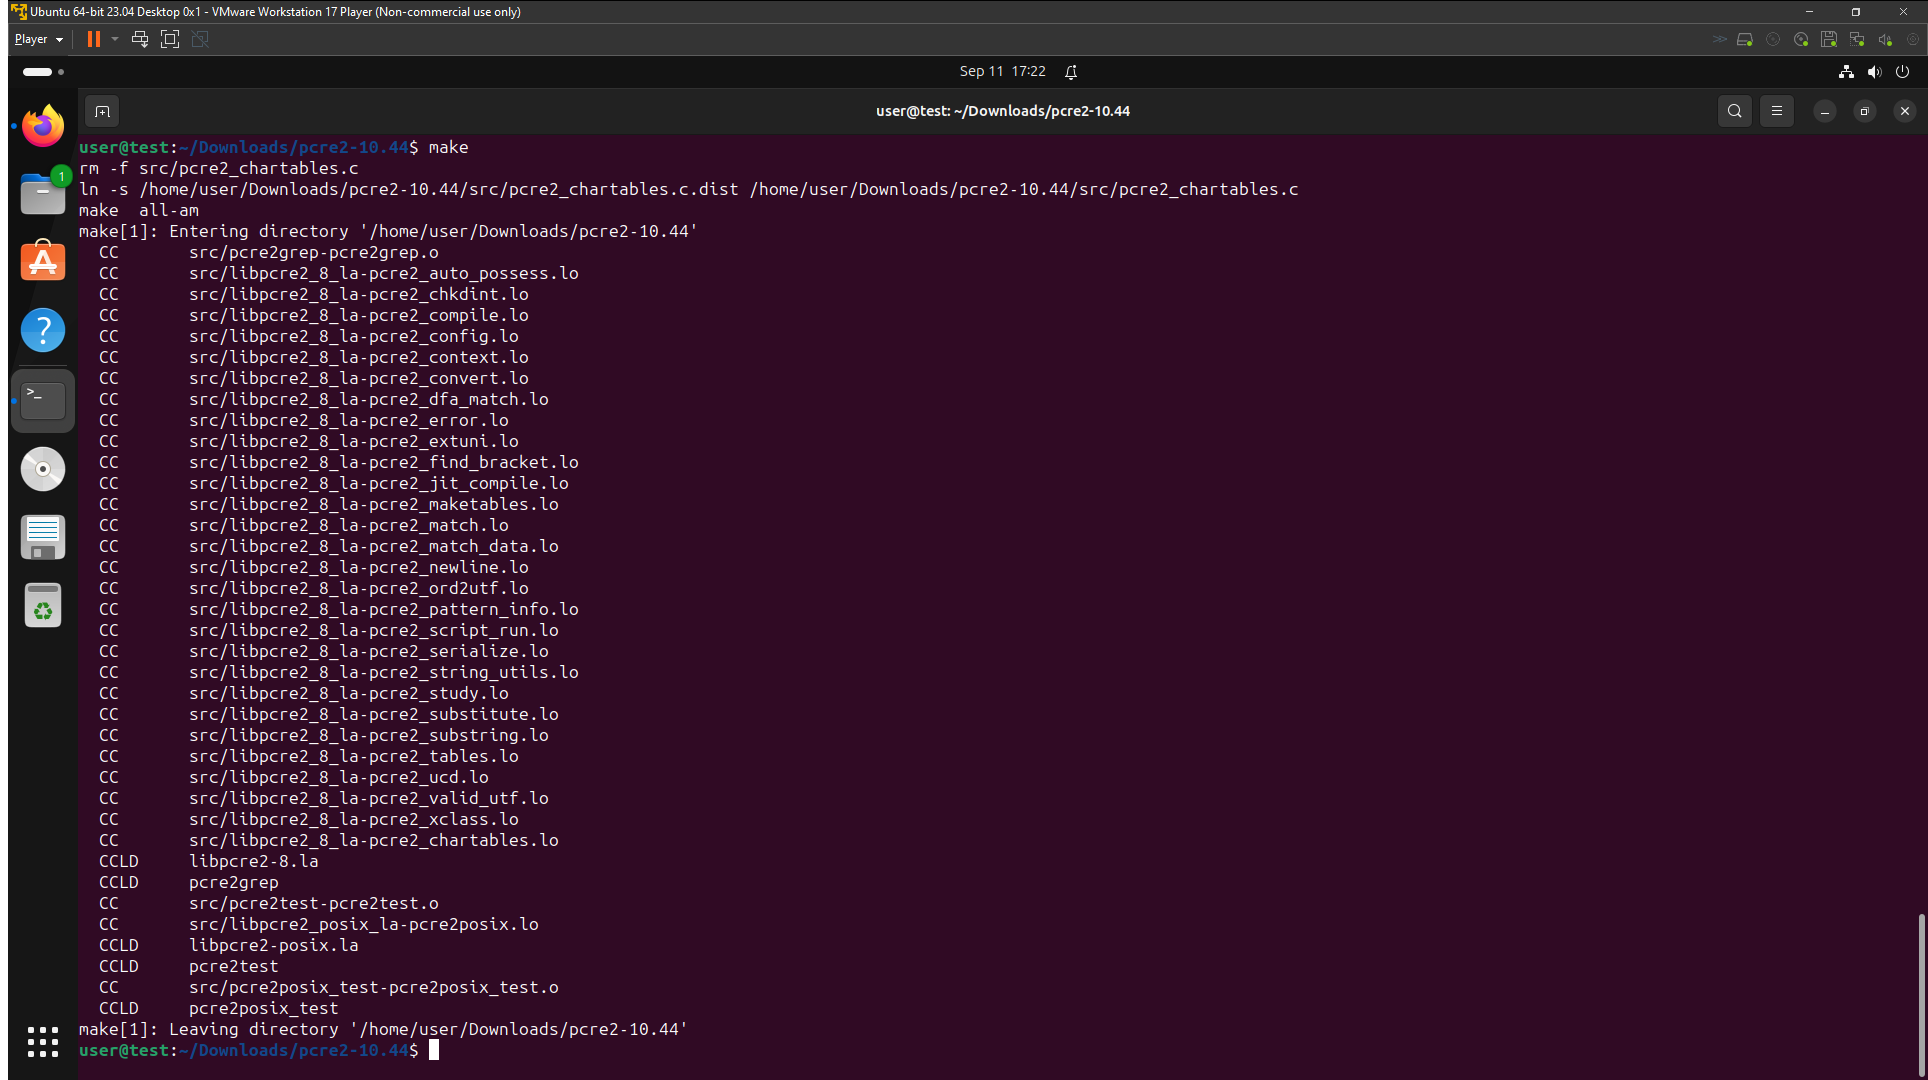
\includegraphics[width=0.9\textwidth]{../figure/pcre2_build_7.png}
        \caption*{Result of building \texttt{pcre2}.}
    \end{figure}

\end{frame}

\subsection{Resolve dependency issue}

\begin{frame}
    \frametitle{Exercise: Build \texttt{json-c}}

    Step 1: Download, uncompress, and examine the content of the project.

    \begin{figure}[H]
        \centering
        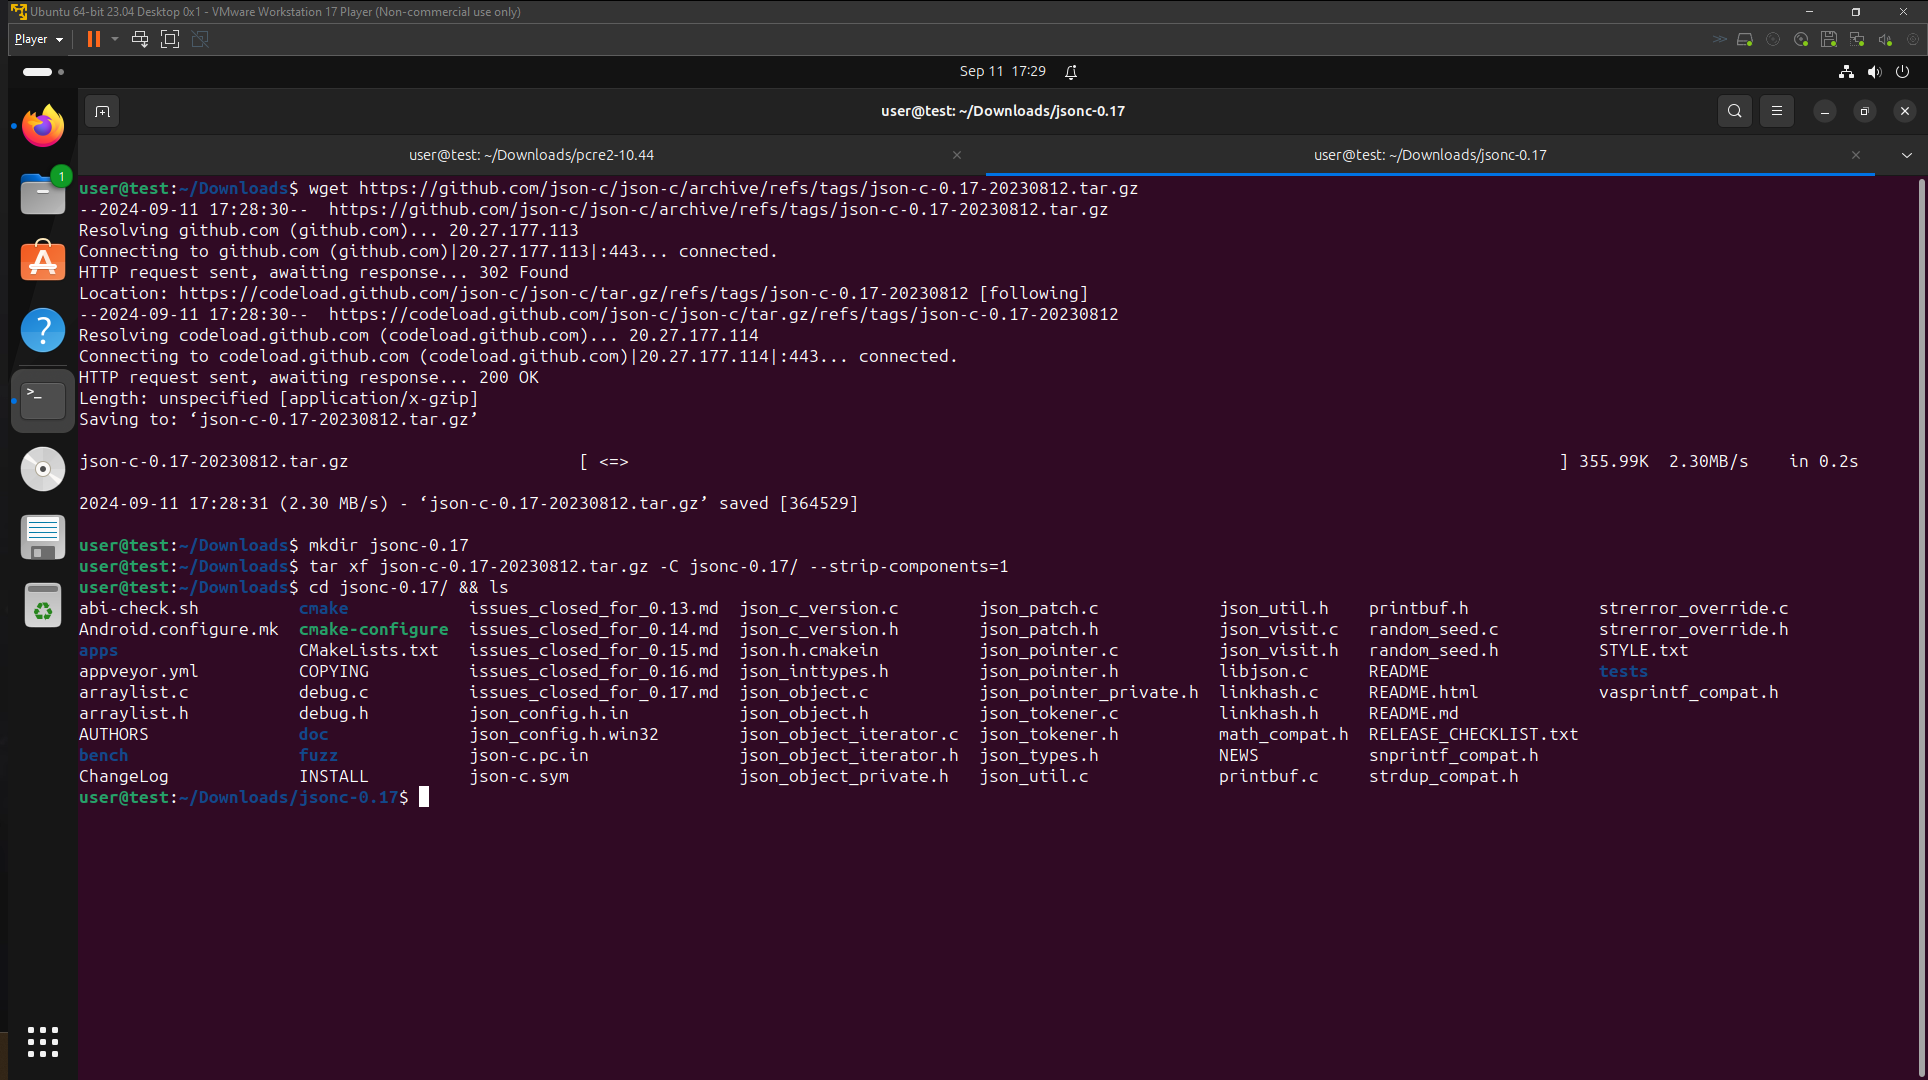
\includegraphics[width=0.9\textwidth]{../figure/jsonc_build_1.png}
    \end{figure}
\end{frame}

\begin{frame}
    \frametitle{Exercise: Build \texttt{json-c}}

    Step 2: Check \texttt{INSTALL} and \texttt{README.md} for installation steps.

    \begin{figure}[H]
        \centering
        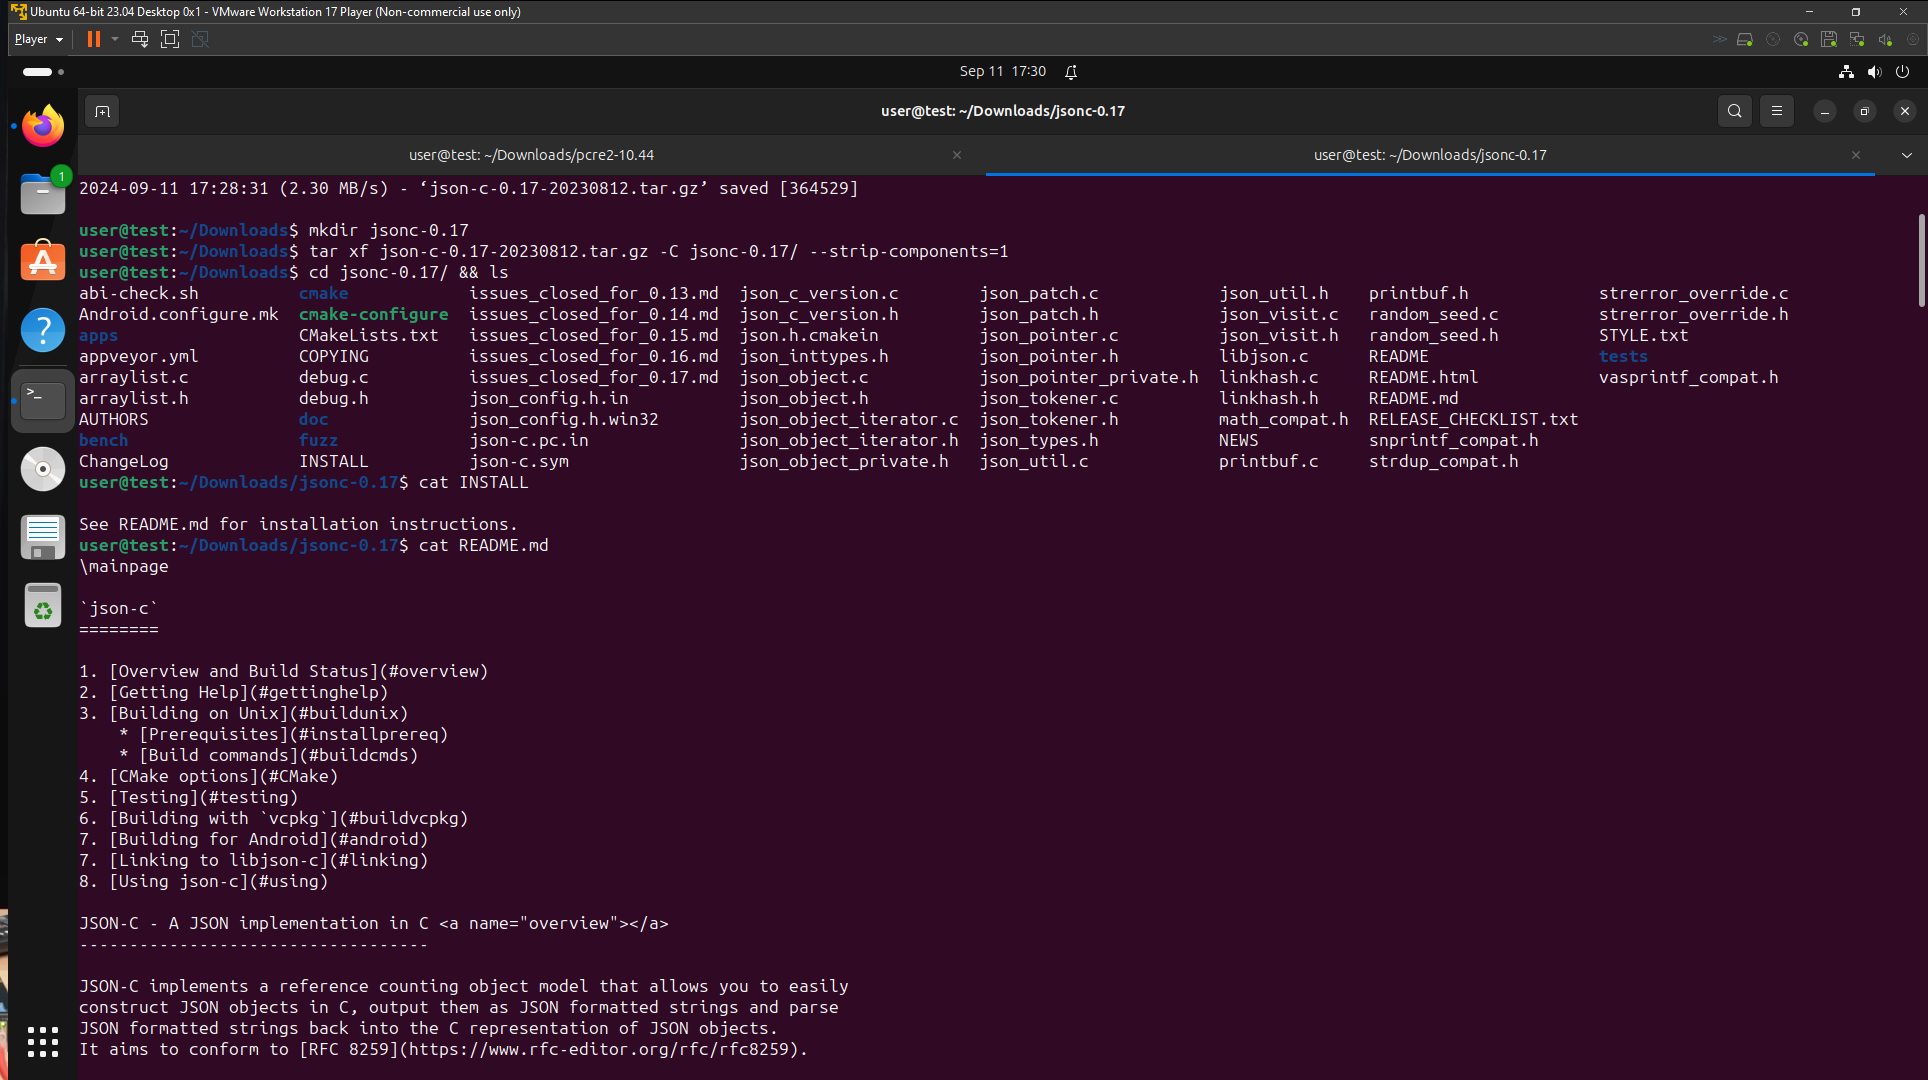
\includegraphics[width=0.9\textwidth]{../figure/jsonc_build_2.png}
    \end{figure}
\end{frame}

\begin{frame}
    \frametitle{Exercise: Build \texttt{json-c}}

    Step 3: Locate official installation steps.

    \begin{figure}[H]
        \centering
        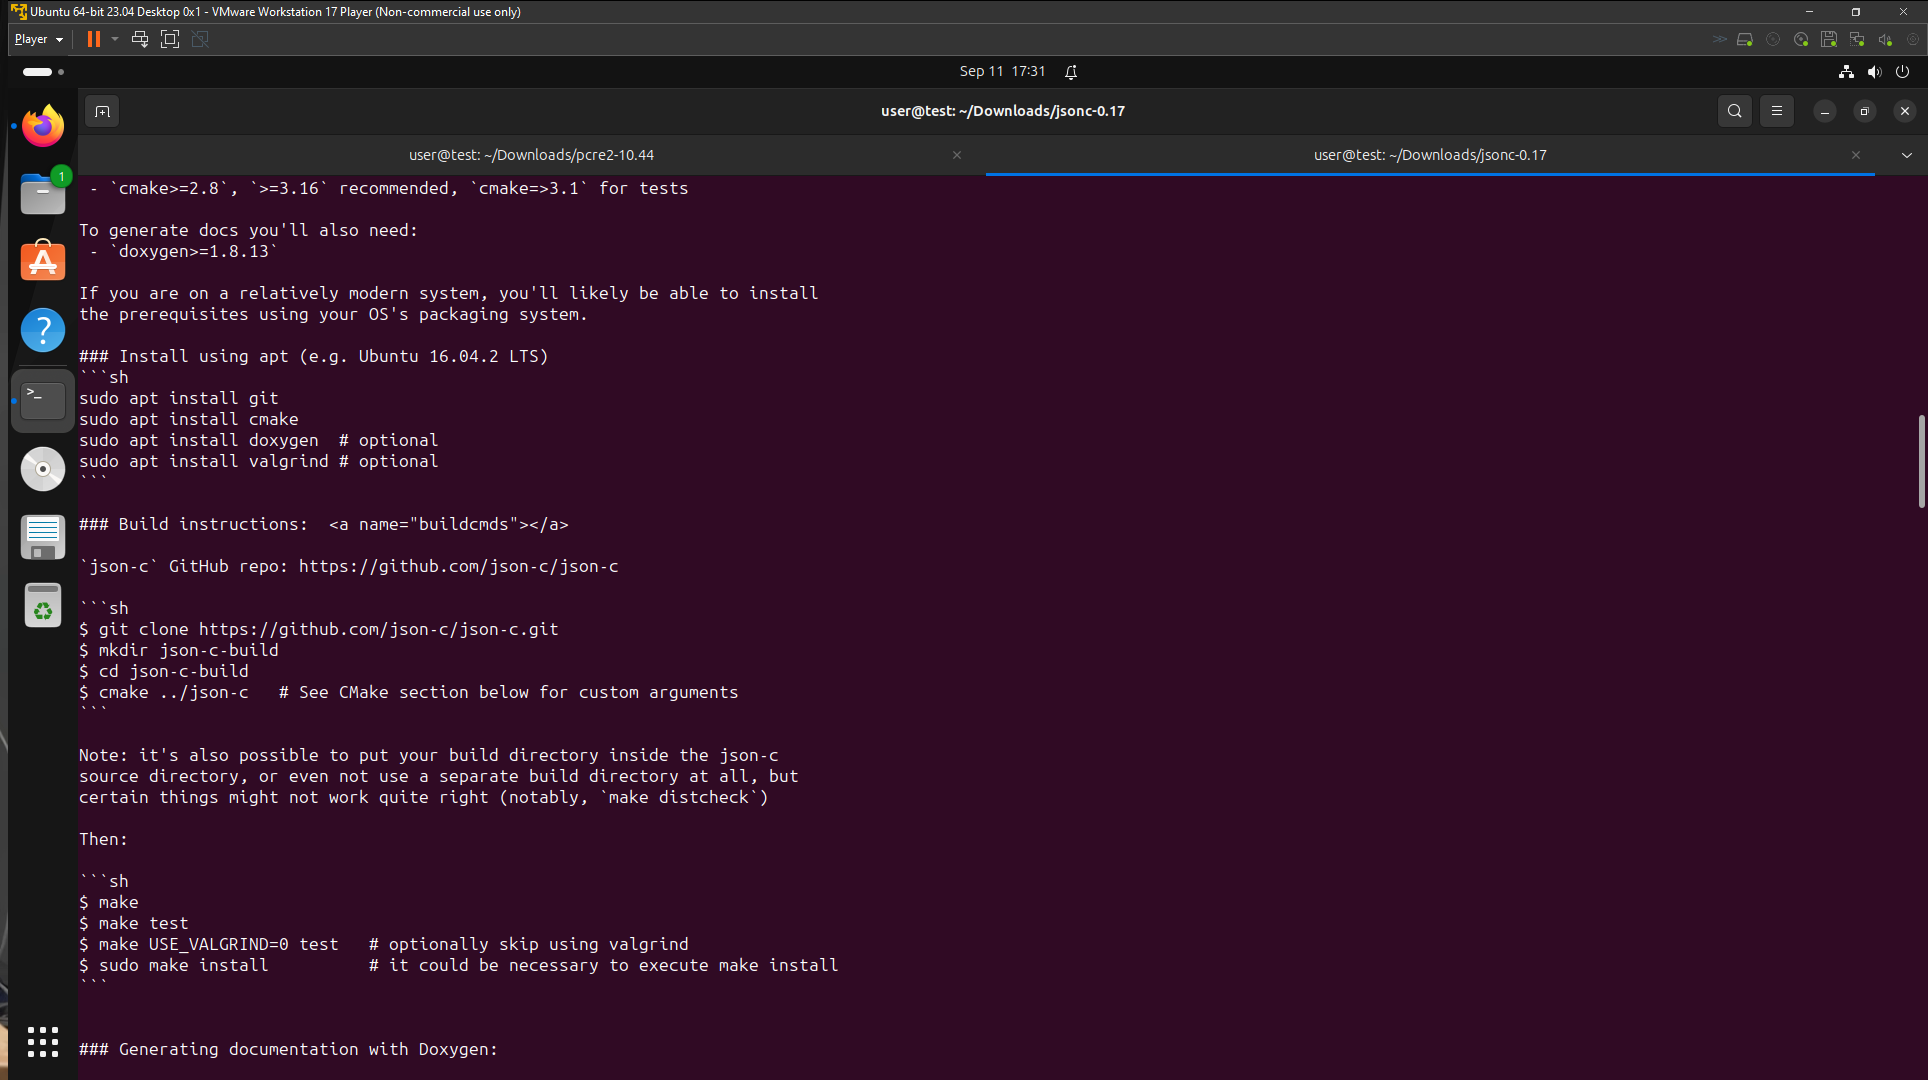
\includegraphics[width=0.9\textwidth]{../figure/jsonc_build_3.png}
    \end{figure}
\end{frame}

\begin{frame}
    \frametitle{Exercise: Build \texttt{json-c}}

    Step 4: Follows the installation steps.

    \begin{figure}[H]
        \centering
        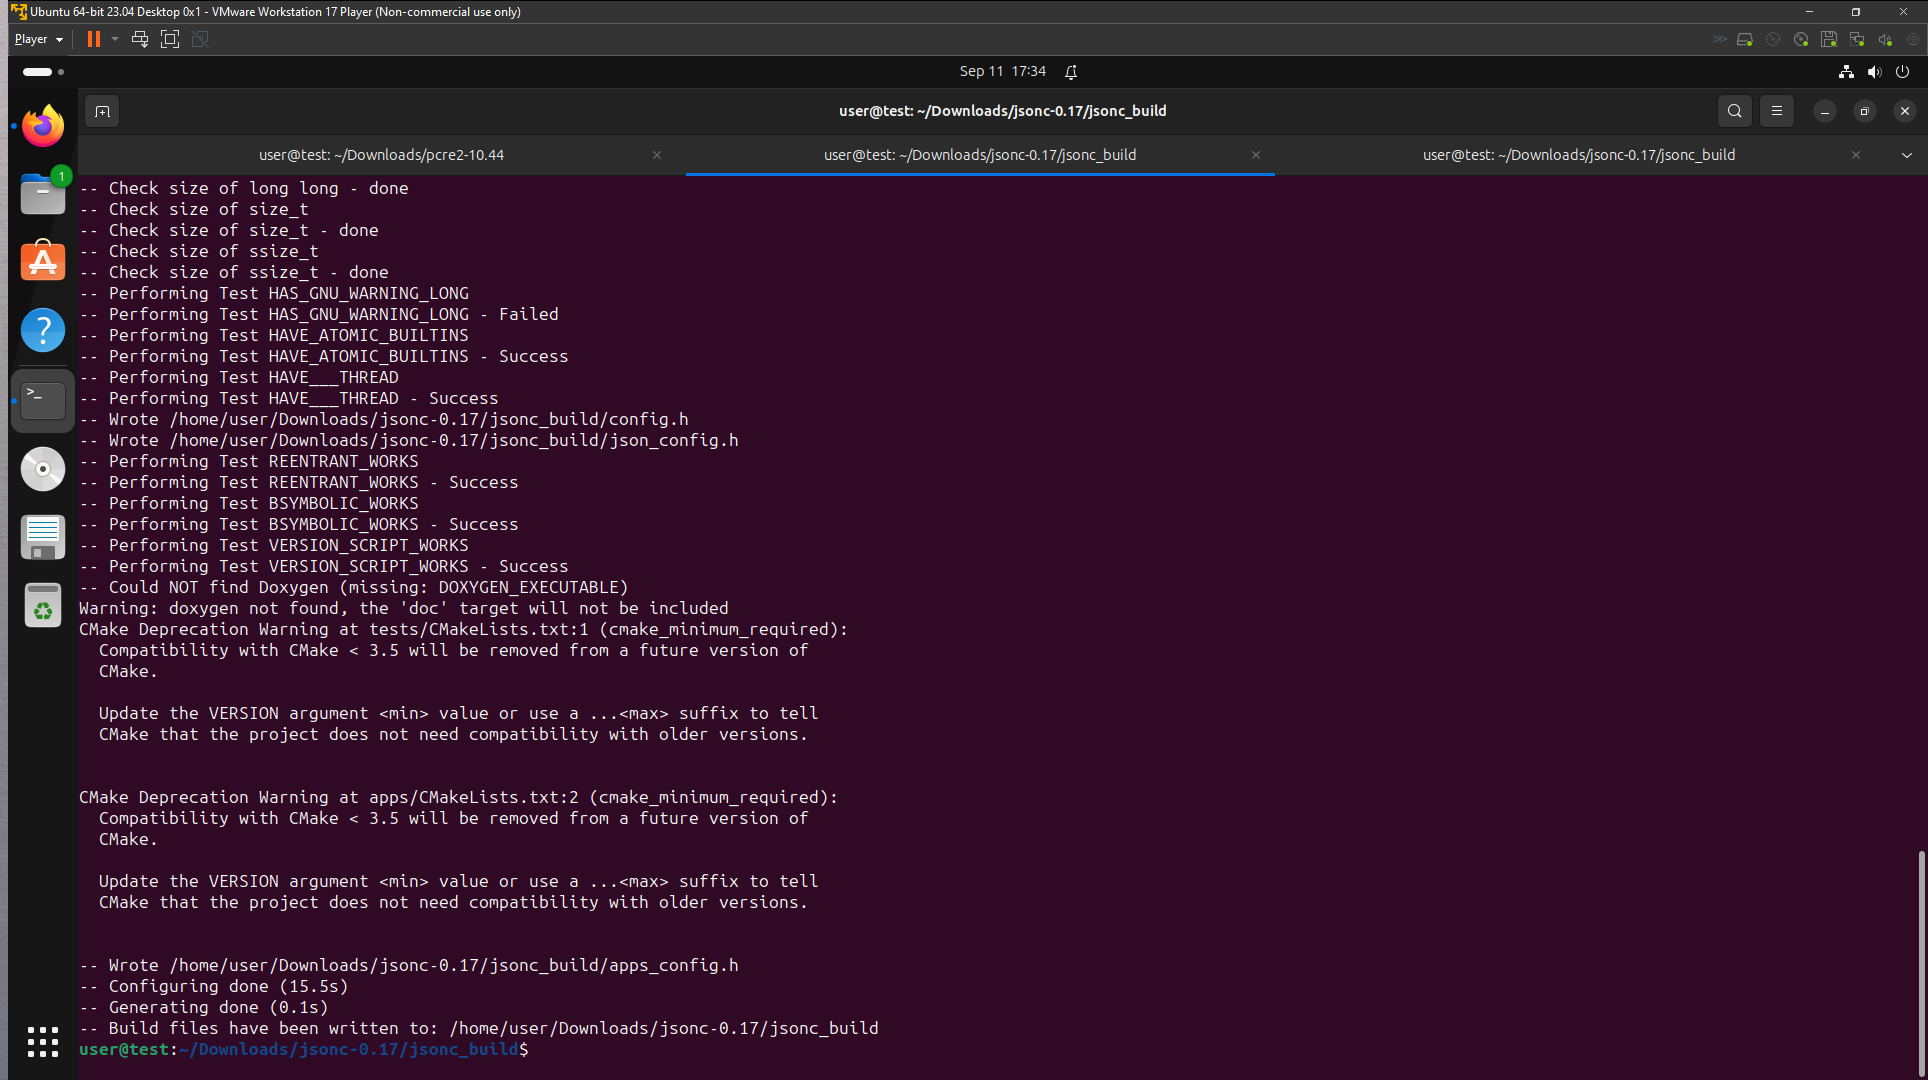
\includegraphics[width=0.9\textwidth]{../figure/jsonc_build_4.png}
        \caption*{Executed \texttt{mkdir jsonc\_build \&\& cd json\_cbuild \&\& cmake ..}}
    \end{figure}
\end{frame}

\begin{frame}
    \frametitle{Exercise: Build \texttt{json-c}}

    Notice there are two warnings indicating dependency issues. 

    \begin{itemize}
        \item \alert{\texttt{doxygen not found}}: Find the distribution of doxygen and install it.
        \item \alert{\texttt{CMake deprecation}}: Update CMake version or compile CMake from source for the latest version.
    \end{itemize}

    These kinds of problems can appear frequently. But make sure to check whether the corresponding \texttt{*.pc} files of dependency exists in default location. Sometimes the build system will not install the \texttt{*.pc} files (especially Meson), making other build systems cannot find the required dependency with \alert{\texttt{pkg-config}}.
\end{frame}

\begin{frame}
    \frametitle{Exercise: Build \texttt{json-c}}

    Step 5: Build the project. (The warnings are skipped)

    \begin{figure}[H]
        \centering
        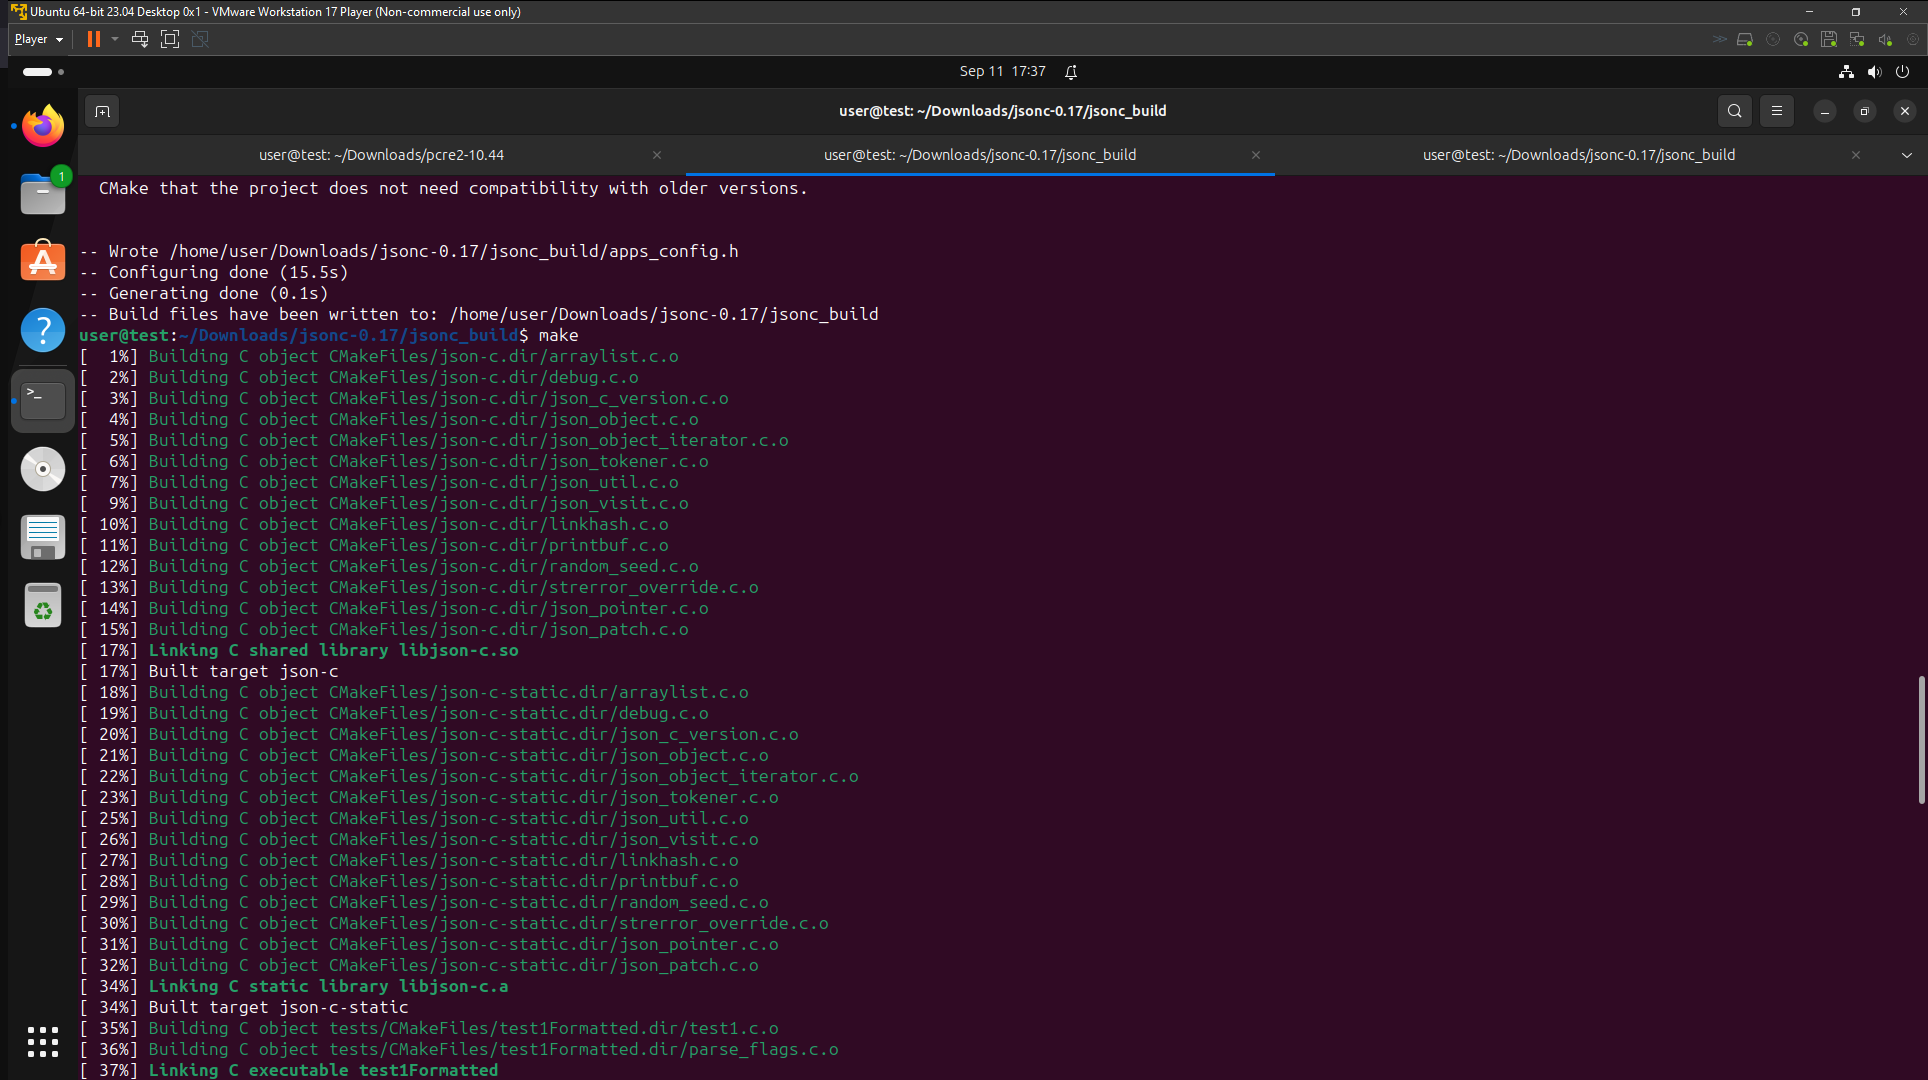
\includegraphics[width=0.9\textwidth]{../figure/jsonc_build_5.png}
    \end{figure}
\end{frame}

\begin{frame}
    \frametitle{Exercise: Build \texttt{json-c}}

    Finally, the build process is finished.

    \begin{figure}[H]
        \centering
        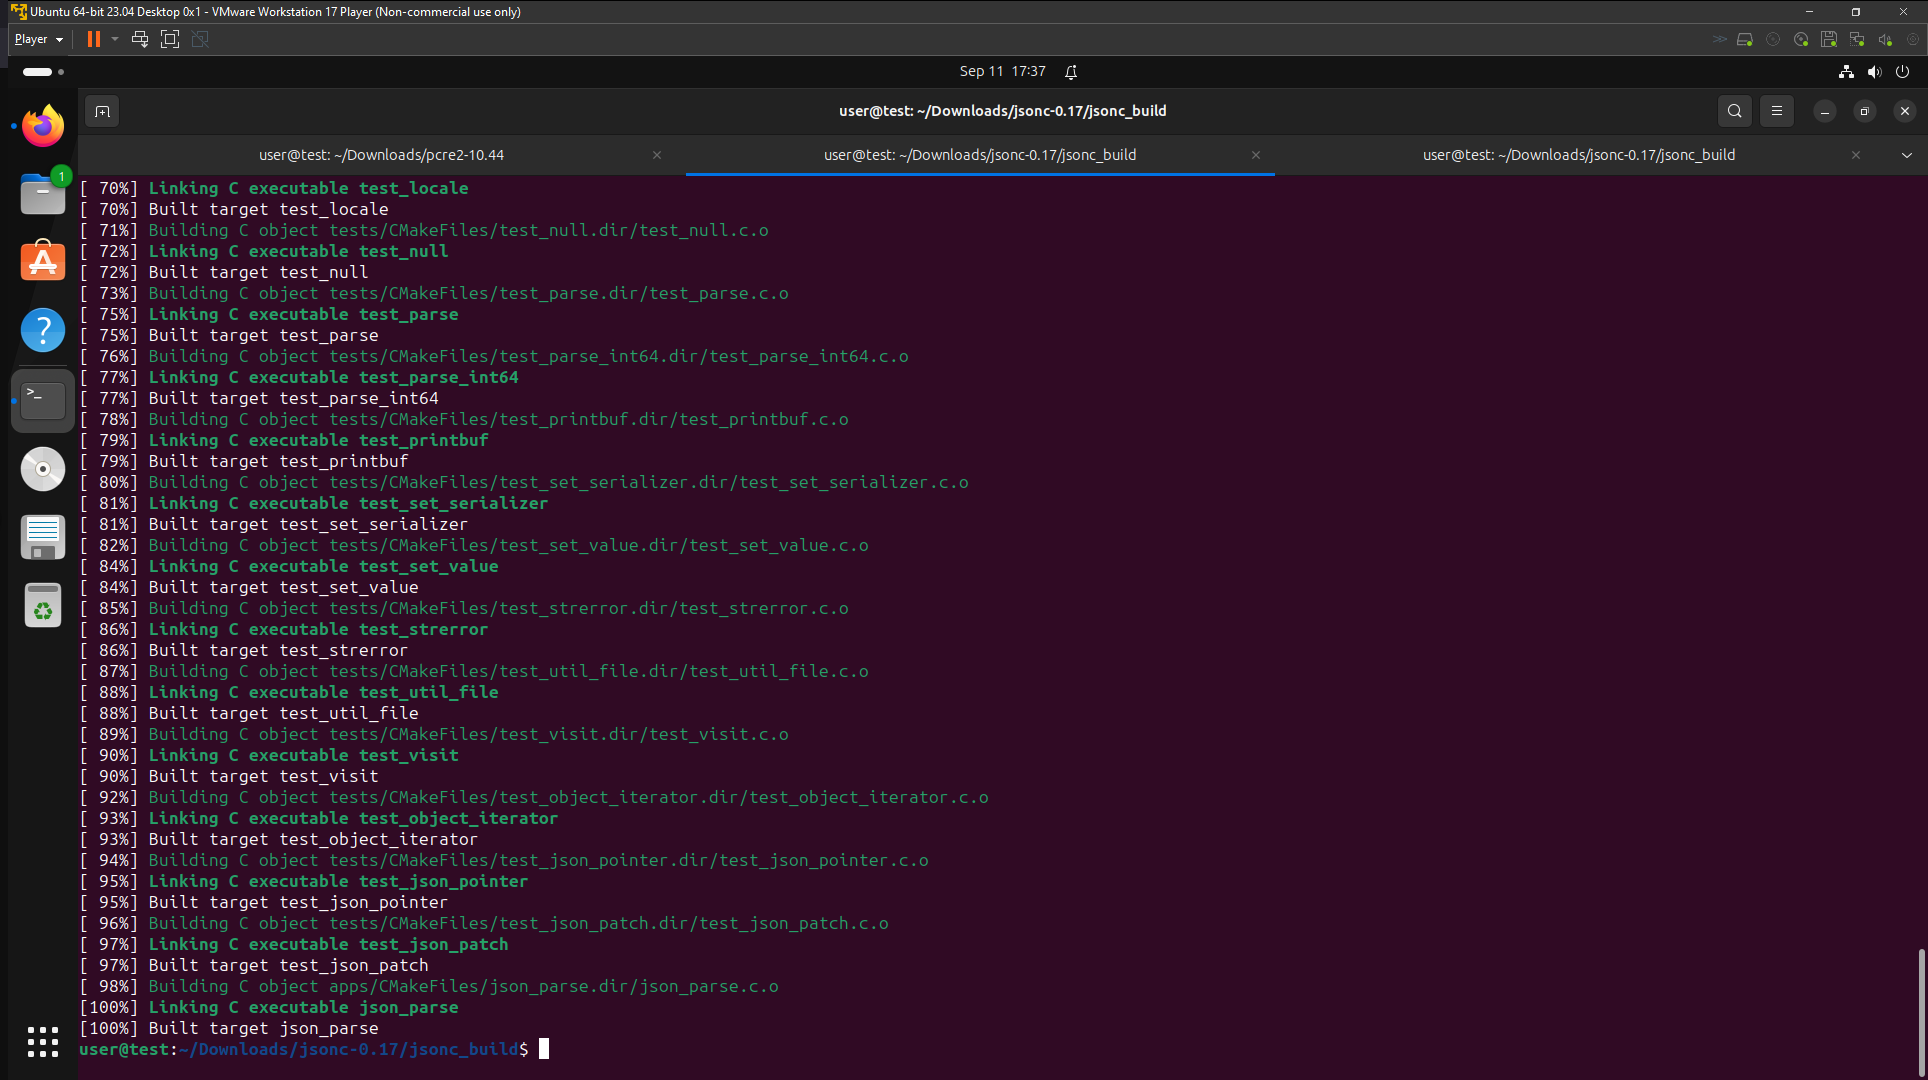
\includegraphics[width=0.9\textwidth]{../figure/jsonc_build_6.png}
    \end{figure}
\end{frame}

\begin{frame}
    \frametitle{Reference}

    \begin{itemize}
        \item \href{https://www.youtube.com/watch?v=YtiPCPtmZrs}{{[}Day 16{]} - Static and Dynamic Libraries (ar, objdump, ld, ldd) - Crash Course in C Programming by Mike Shah}
        \item \href{https://www.youtube.com/watch?v=Slfwk28vhws}{Write Better Code! | How to Create Shared Libraries in C/C++}
        \item \href{https://docs.redhat.com/en/documentation/red_hat_enterprise_linux/6/html/developer_guide/cmd-autotools-upstreamdocs\#cmd-autotools-upstreamdocs}{Red Hat Documentation 3.2.3. Autotools Documentation}
    \end{itemize}
\end{frame}
